\documentclass[12pt]{extarticle}
%Some packages I commonly use.
\usepackage[italian]{babel}
\usepackage{graphicx}
\usepackage{framed}
\usepackage[normalem]{ulem}
\usepackage{amsmath}
\usepackage{amsthm}
\usepackage{amssymb}
\usepackage{amsfonts}
\usepackage{enumerate}
\usepackage{url}
\usepackage{hyperref}
\usepackage[utf8]{inputenc}
\usepackage[top=1 in,bottom=1in, left=1 in, right=1 in]{geometry}
\usepackage{comment}
\usepackage[export]{adjustbox}
\usepackage{wrapfig}
\usepackage{mathtools}
\usepackage{commath}
%\usepackage[sc,osf]{mathpazo}
\usepackage{gensymb} % \degree command (°)
\usepackage{dirtytalk} % \say command ("")
\usepackage{amsfonts}
\usepackage{amstext}
\usepackage{float}
\usepackage[utf8]{inputenc}
\usepackage{graphicx}
\usepackage{verbatim}
\usepackage{afterpage}
\usepackage{imakeidx}
\usepackage{biblatex}
\usepackage{blindtext}
\usepackage{caption}
\usepackage{subcaption}
\usepackage{subfloat}
\usepackage{float}
\usepackage[table]{xcolor}
\usepackage[a4paper,width=150mm,top=25mm,bottom=25mm,bindingoffset=6mm]{geometry}
\usepackage{listings}
\usepackage{color}
\definecolor{dkgreen}{rgb}{0,0.8,0}
\definecolor{gray}{rgb}{0.5,0.5,0.5}
\definecolor{mauve}{rgb}{0.58,0,0.82}
\lstset{frame=shadowbox,
  language=Matlab,
  aboveskip=3mm,
  belowskip=3mm,
  showstringspaces=false,
  columns=flexible,
  basicstyle={\small\ttfamily},
  numbers=none,
  numberstyle=\tiny\color{gray},
  keywordstyle=\color{blue},
  commentstyle=\color{dkgreen},
  stringstyle=\color{mauve},
  breaklines=true,
  breakatwhitespace=true,
  tabsize=3
}
\usepackage[framed,useliterate]{mcode} % after "framed" you can put also "numbered" for line numbers, and "autolinebreaks" for '...'

%A bunch of definitions that make my life easier
\newcommand{\matlab}{{\sc Matlab} }
\newcommand{\cvec}[1]{{\mathbf #1}}
\newcommand{\rvec}[1]{\vec{\mathbf #1}}
\newcommand{\ihat}{\hat{\textbf{\i}}}
\newcommand{\jhat}{\hat{\textbf{\j}}}
\newcommand{\khat}{\hat{\textbf{k}}}
\newcommand{\minor}{{\rm minor}}
\newcommand{\trace}{{\rm trace}}
\newcommand{\spn}{{\rm Span}}
\newcommand{\rem}{{\rm rem}}
\newcommand{\ran}{{\rm range}}
\newcommand{\range}{{\rm range}}
\newcommand{\mdiv}{{\rm div}}
\newcommand{\proj}{{\rm proj}}
\newcommand{\R}{\mathbb{R}}
\newcommand{\N}{\mathbb{N}}
\newcommand{\Q}{\mathbb{Q}}
\newcommand{\Z}{\mathbb{Z}}
\newcommand{\<}{\langle}
\renewcommand{\>}{\rangle}
\renewcommand{\emptyset}{\varnothing}
\newcommand{\attn}[1]{\textbf{#1}}
\theoremstyle{definition}
\newtheorem{theorem}{Theorem}
\newtheorem{corollary}{Corollary}
\newtheorem*{definition}{Definition}
\newtheorem*{example}{Example}
\newtheorem*{note}{Note}
\newtheorem{exercise}{Exercise}
\newcommand{\bproof}{\bigskip {\bf Proof. }}
\newcommand{\eproof}{\hfill\qedsymbol}
\newcommand{\Disp}{\displaystyle}
\newcommand{\qe}{\hfill\(\bigtriangledown\)}
\newcommand{\columnvector}[1]{\begin{bmatrix}#1\end{bmatrix}}
\setlength{\columnseprule}{1 pt}


\makeatletter % makes the vertical space in vectors customizable
\renewcommand*\env@matrix[1][\arraystretch]{%
  \edef\arraystretch{#1}%
  \hskip -\arraycolsep
  \let\@ifnextchar\new@ifnextchar
  \array{*\c@MaxMatrixCols c}}
\makeatother

\addbibresource{biblio/Multiple Model Adaptive Complementary Filter for Attitude Estimation.bib}
\addbibresource{biblio/Comparison.bib}
\addbibresource{biblio/MPU6050.bib}
\addbibresource{biblio/MPU9250.bib}
\addbibresource{biblio/tilt-compensated ecompass.bib}
\addbibresource{biblio/calibrating ecompass.bib}
\addbibresource{biblio/ahrs.bib}


\begin{document}

%Copertina

\title{Progetto del corso di Sistemi di Guida e Navigazione}
\author{
  Ilaria Martelli\\
}
\date{\today}

\begin{figure}[htp]

\includegraphics[scale=0.8]{immagini/unipi.png}
\centering
\end{figure}

\begin{center}
\sc\centering\onehalfspacing\fontsize{4mm}{6mm}\selectfont Dipartimento di Ingegneria Dell'Informazione\\Corso di Ingegneria Robotica e dell'Automazione\\
\end{center}
\begin{center}
\vspace{2cm}

\Huge\bfseries\sc Sistemi di Guida e Navigazione\\[1cm] \bfseries\Large\sc Relazione:\\ AHRS sensor-based\\ Motion Tracking Glove %[0.3cm]\normalsize\sc Subtitle\\ 
\end{center}
\vspace{2cm}


\begin{center}
Ilaria Martelli\\
Luca Ricci\\
\vspace{0.5cm}
\today
\end{center}
\clearpage
 \tableofcontents
 \clearpage


\section{Contenuto dell'analisi e obiettivi}

Lo scopo di questo progetto è la sintesi di un sistema di filtraggio dati di un complesso multi-IMU situato sul dito di un guanto indossabile per ricostruire la posa cinematica \cite{8624929} e visualizzare una replica virtuale in tempo reale tramite Unity.\\

L'elaborato è diviso in 3 fasi principali:
\begin{enumerate}
    \item lettura dei dati raccolti dalle IMU e spedizione tramite seriale (programma utilizzato: Arduino);
    \item filtro che elabora i dati ricevuti da IMU per restituirne l'assetto (linguaggio utilizzato: Python);
    \item rappresentazione tridimensionale di una mano, che utilizza le misure di assetto trovate per posizionarsi in modo da seguire i movimenti del guanto (programma utilizzato: Unity).
\end{enumerate}


\begin{figure}[H]
    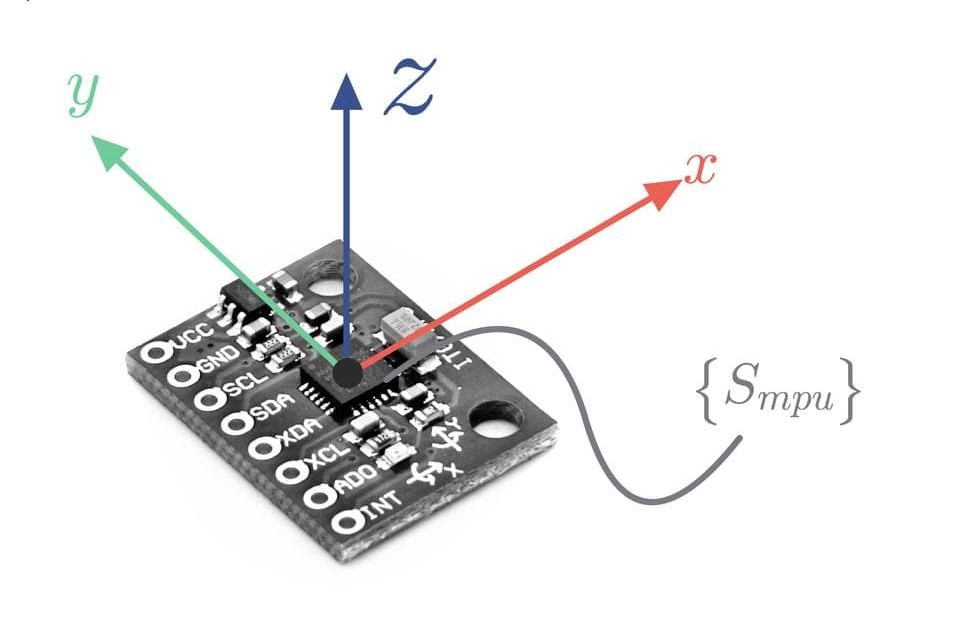
\includegraphics[scale=0.35]{immagini/IMU_sdr.jpg}
    \centering
    \caption{Sistemi di riferimento \textit{body} su una IMU.}
\end{figure}

\clearpage
\section{Descrizione del sistema}\label{Descrizione del sistema}

\subsection{Materiale utilizzato}

Per il progetto sono state utilizzate:
\begin{enumerate}
    \item una MPU-6050 a 6 gradi di libertà (3\textit{dof accelerometer} + 3\textit{dof gyroscope});
    \item due MPU-9250 a 9 gradi di libertà (3\textit{dof accelerometer} + 3\textit{dof gyroscope} + 3\textit{dof magnetometer});
    \item un multiplexer TCA9548A (per permettere l'utilizzo di più IMU sullo stesso canale I2C);
    \item una scheda ESP32 programmabile con Arduino.
\end{enumerate}

\begin{figure}[H]
    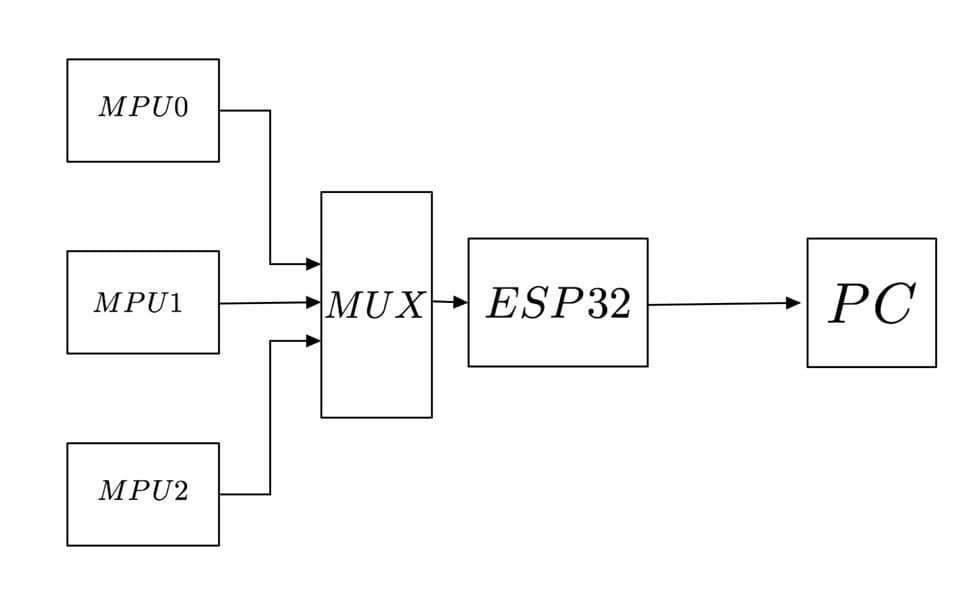
\includegraphics[scale=0.35]{immagini/schema_blocchi.jpg}
    \centering
    \caption{Schema a blocchi complessivo.}
\end{figure}

\clearpage

\subsection{Caratterizzazione IMU}\label{Caratterizzazione IMU}

Una IMU è un'unità di misura inerziale che comprende tre accelerometri e tre giroscopi posti sui tre assi di interesse dell'IMU (assi \textit{body}).

\subsubsection{Dati accelerometro}\label{Dati accelerometro}

\begin{figure}[H]
    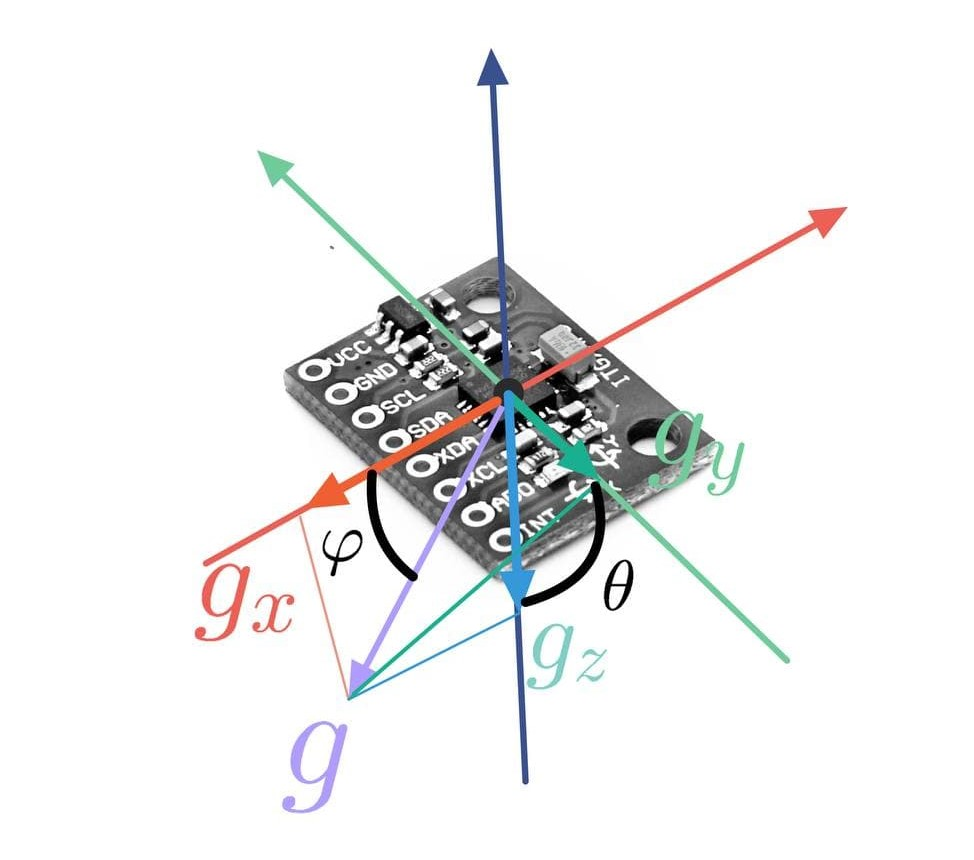
\includegraphics[scale=0.35]{immagini/IMU_sdr_g.jpg}
    \centering
    \caption{Accelerometro.}
\end{figure}

Attraverso i dati dell'accelerometro, si può inferire l'inclinazione di roll (rotazione attorno all'asse x) e pitch (rotazione attorno all'asse y) dell'IMU, considerando i valori trovati sui tre assi locali (\textit{body}) come le componenti parziali del vettore gravità, che sappiamo puntare verso il basso in assi fissi (\textit{navigation}).

\begin{equation}\label{eq phi roll acc}
    \phi_a = \tan^{-1} \begin{pmatrix} \frac{a_y}{a_z} \end{pmatrix}
\end{equation}
\begin{equation}\label{eq theta pitch acc}
    \theta_a = \tan^{-1} \begin{pmatrix} \frac{-a_x}{a_y \sin{\phi_a} \, + \, a_z \cos{\phi_a}} \end{pmatrix}
\end{equation}

D'altra parte, usare solo le misure date dagli accelerometri genera errori nel caso in cui l'IMU, invece che venire ruotata, sia sottoposta a un'accelerazione data da un moto lineare: in tal caso, questo metodo riporterebbe rotazioni che non esistono. Per questo è necessario filtrare le misure con altri sensori, in modo che gli errori di uno vengano compensati dagli altri (la cosiddetta \textit{sensor fusion}).

\clearpage

\subsubsection{Dati giroscopio}\label{Dati giroscopio}

\begin{figure}[H]
    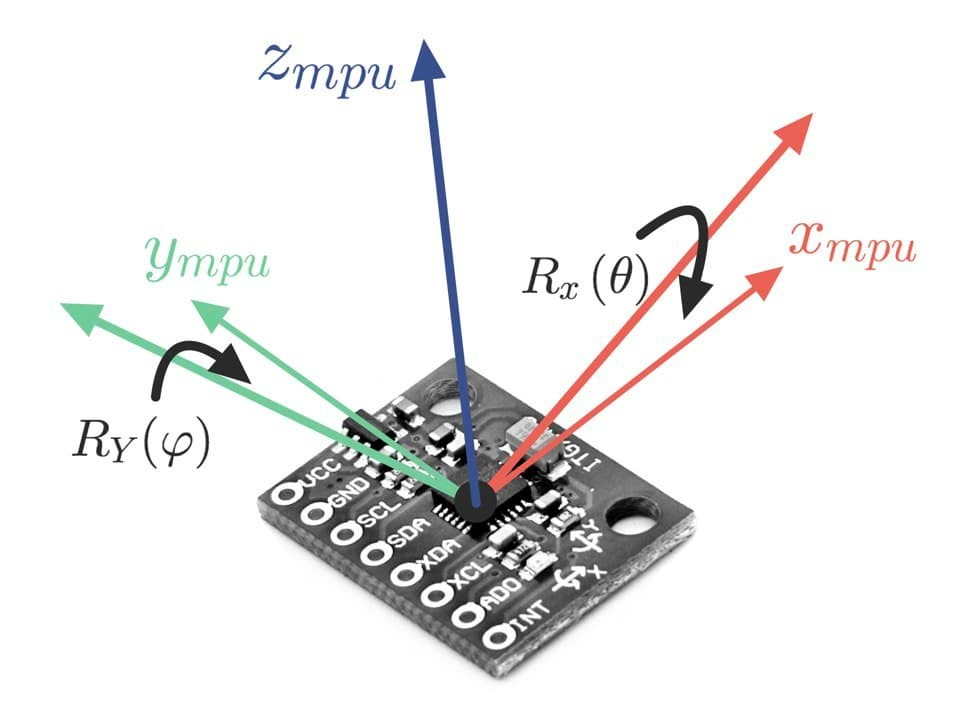
\includegraphics[scale=0.25]{immagini/IMU_sdr_R.jpg}
    \centering
    \caption{Giroscopio.}
\end{figure}

Allo stesso modo dell'accelerometro, il giroscopio può trovare la velocità angolare sui tre assi di riferimento. In questo caso, una semplice operazione di integrazione ci consente di ricavare gli angoli relativi nel tempo, che poi vengono sommati alla loro misura precedente.\\
Questo metodo necessita la conoscenza dell'orientazione iniziale dell'IMU, ma tale richiesta viene soddisfatta ponendo gli angoli iniziali a 0 e facendo partire il programma che invia i dati quando il guanto è parallelo al suolo (roll e pitch nulli).

\begin{equation*}
    \dot{q}_{gyro} = \frac{1}{2} \, \Omega_t \, q
\end{equation*}
\begin{equation*}
	q_{gyro} = q + \dot{q}_{gyro} \, dt
\end{equation*}\label{integr gyro}

\begin{figure}[H]
    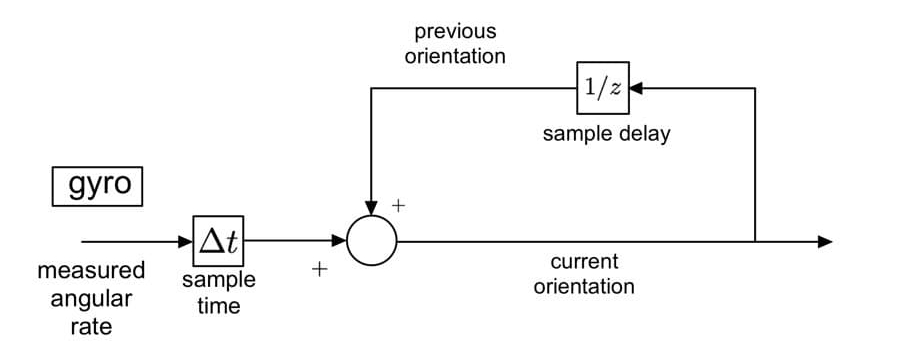
\includegraphics[scale=0.35]{immagini/photo_2022-03-07_09-40-18.jpg}
    \centering
    \caption{Elaborazione dati giroscopio.}
\end{figure}

Per l'integrazione delle misure delle velocità angolari, sono state usate le formule (\ref{integr phi}), (\ref{integr theta}) e (\ref{integr psi}), che combinano sia la semplice operazione di integrazione con una rotazione rispetto agli angoli dello step precedente, in modo che i sistemi di riferimento tra angoli trovati con accelerometro-magnetometro e giroscopio siano allineati.

\begin{equation}\label{integr phi}
    \dot{\phi} = p + q \sin{\phi} \tan{\theta} + r \cos{\phi} \tan{\theta}
\end{equation}

\begin{equation}\label{integr theta}
    \dot{\theta} = q \cos{\phi} - r \sin{\phi}
\end{equation}

\begin{equation}\label{integr psi}
    \dot{\psi} = q \sin{\phi} \sec{\theta} + r \cos{\phi} \sec{\theta}
\end{equation}\\

Un problema più grave invece è la considerazione dell'errore del giroscopio nel tempo: poiché la misura della velocità angolare è sottoposta a rumore, integrare tale misura contribuisce al \textit{drifting}, ovvero una forma di alterazione della misura in cui l'angolo ricavato aumenta nel tempo anche se l'IMU rimane ferma.\\
Per risolvere il \textit{drifting} si usa la misura ricavata dall'accelerometro come correzione.

\clearpage

\subsection{Caratterizzazione AHRS}

Un AHRS (talvolta chiamato MARG per \textit{Magnetic, Angular Rate and Gravity}) è un sistema di riferimento di orientazione e direzione che include una IMU e un magnetometro.\\
In particolare, le MPU-9250 usate hanno come base un'IMU uguale alle MPU-6050 a cui è stato aggiunto un magnetometro AK8963 a 3 gradi di libertà.

\subsubsection{Dati magnetometro}\label{Dati magnetometro}

\begin{figure}[H]
    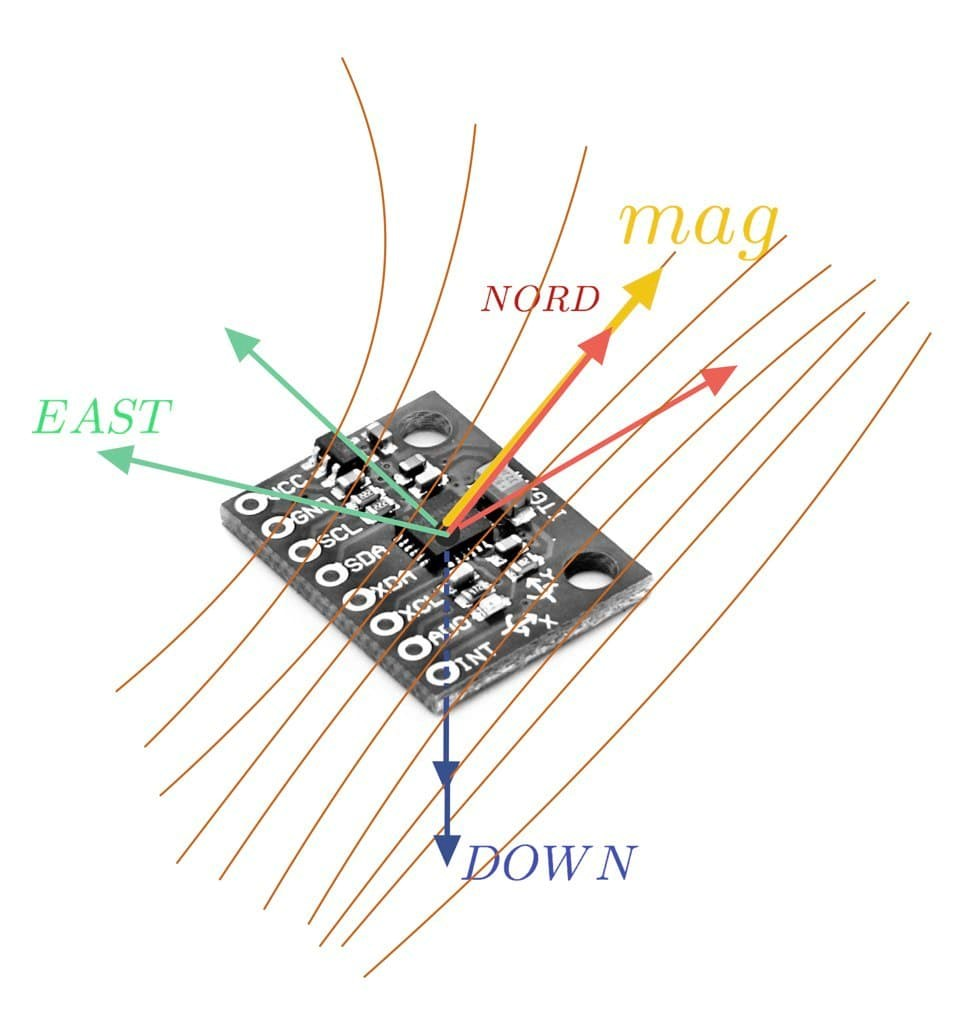
\includegraphics[scale=0.25]{immagini/IMU_sdr_magn.jpg}
    \centering
    \caption{Magnetometro.}
\end{figure}

Nelle AHRS ad accelerometro e giroscopio delle IMU si aggiunge la misura di \textit{heading} data dal magnetometro, che permette di ricavare anche lo yaw (rotazione attorno all'asse z) del dispositivo.\\

I passaggi sono i seguenti: si ruotano i dati ricevuti dal magnetometro ($m$) utilizzando i valori di roll e pitch già ricavati dall'accelerometro, e da essi si ricava lo yaw.
\begin{equation*}
    \begin{bmatrix} b_x\\ b_y\\ b_z \end{bmatrix} = R_y(\theta_a) R_x(\phi_a) \begin{bmatrix} m_x\\ m_y\\ m_z \end{bmatrix}
\end{equation*}
\begin{equation*}
    \psi_m = \tan^{-1} \begin{pmatrix} \frac{-b_y}{b_x} \end{pmatrix}
\end{equation*}
Da cui risulta
\begin{equation}\label{eq psi yaw magn}
    \psi_m = \tan^{-1} \begin{pmatrix} \frac{m_x \sin{\phi_a} \, - \, m_y \cos{\phi_a}}{m_x \cos{\theta_a} \, + \, m_y \sin{\theta_a} \sin{\phi_a} \, + \, m_z \sin{\theta_a} \cos{\phi_a}} \end{pmatrix}
\end{equation}

\clearpage

\subsection{Posizionamento delle IMU}

\begin{figure}[H]
    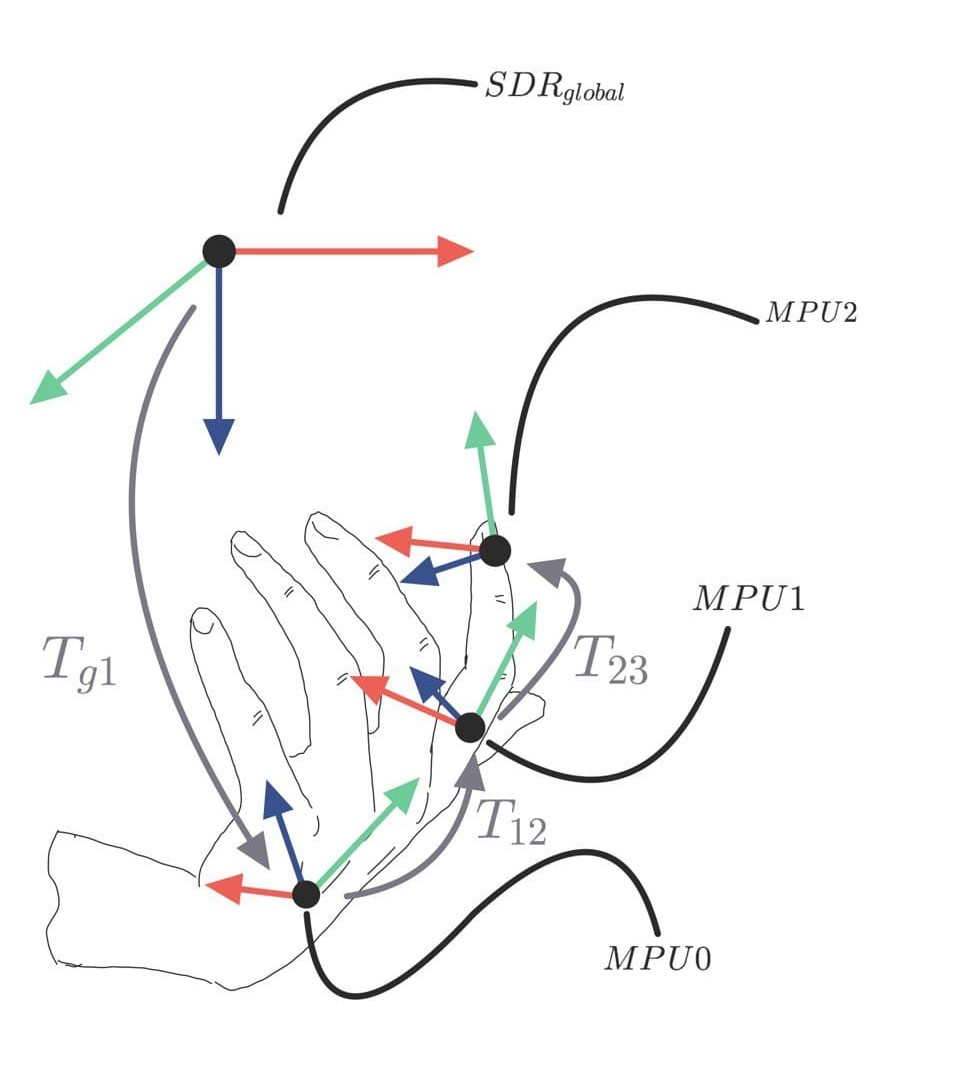
\includegraphics[scale=0.25]{immagini/guanto_sdr.jpg}
    \centering
    \caption{Sistemi di riferimento del dito.}
\end{figure}

Le MPU-9250, essendo provviste di magnetometro per misurare l'\textit{heading}, sono state poste una sul dorso della mano (MPU0), per poterne visualizzare lo yaw, e una sulla falange prossimale, ovvero quella più vicina al palmo (MPU1), in modo da poter visualizzare rotazioni relative tra il dito e il palmo della mano. La MPU-6050 è stata invece posizionata sulla falange distale, ovvero quella più vicina alla punta del dito (MPU2).\\

\begin{figure}[H]
    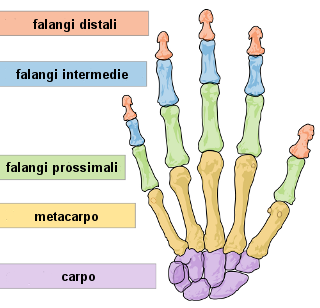
\includegraphics[scale=0.45]{immagini/falangi.png}
    \centering
    \caption{Falangi di una mano.}
\end{figure}

\clearpage
\section{Implementazione hardware}

La fase di sviluppo di questo progetto ha subito molti problemi nella parte hardware, portando a vari prototipi e infine alla riduzione della complessità del progetto stesso.\\

Infatti si è passati da un sistema di sensorizzazione completa di una mano, con 2 IMU per dito più 3 IMU per modellare il movimento del palmo (in particolare il piegamento sul metacarpo dato dal pollice e quello dato dal mignolo), per un totale di 13 IMU e 2 multiplexer, a un progetto semplificato su un singolo dito, per un totale di 3 IMU e 1 multiplexer.

\subsection{Primo prototipo}

\begin{figure}[H]
    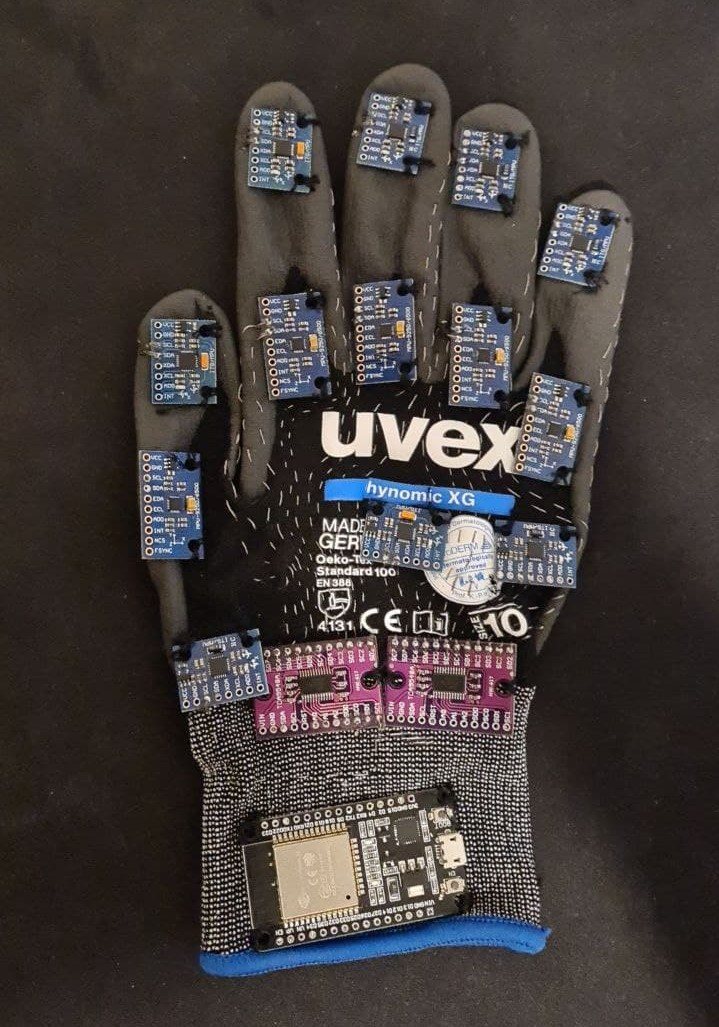
\includegraphics[scale=0.35]{immagini/prototipo1.jpg}
    \centering
    \caption{V1}
\end{figure}

Inizialmente si era pensato di utilizzare un filo conduttivo per collegare insieme i dispositivi posti sul guanto: questo avrebbe consentito di cucire più saldamente i vari componenti, utilizzando sia cuciture normali che il filo conduttivo stesso, e allo stesso tempo avrebbe dato al guanto un aspetto più \textit{tight fit}, non avendo cavi che si estendono oltre il volume del guanto.\\
Purtroppo questa strada ha portato a molti problemi di interferenze tra circuiti troppo vicini, e ancor più grave la presenza di cortocircuiti, tra cui almeno uno sui molteplici fili che collegavano i pin VCC e GND per l'alimentazione delle IMU, causando drastici cali di tensione che permettevano l'accensione di appena 2/3 IMU su 12 (sparse, non sullo stesso dito).\\

Per cercare di risolvere il problema si è ricorsi all'uso di un multimetro per l'individuazione dei cortocircuiti, e una melassa isolante da spalmare sui fili. Siccome anche questo non ha portato ai risultati sperati, si è deciso di ritentare modificando il progetto.

\begin{figure}[H]
    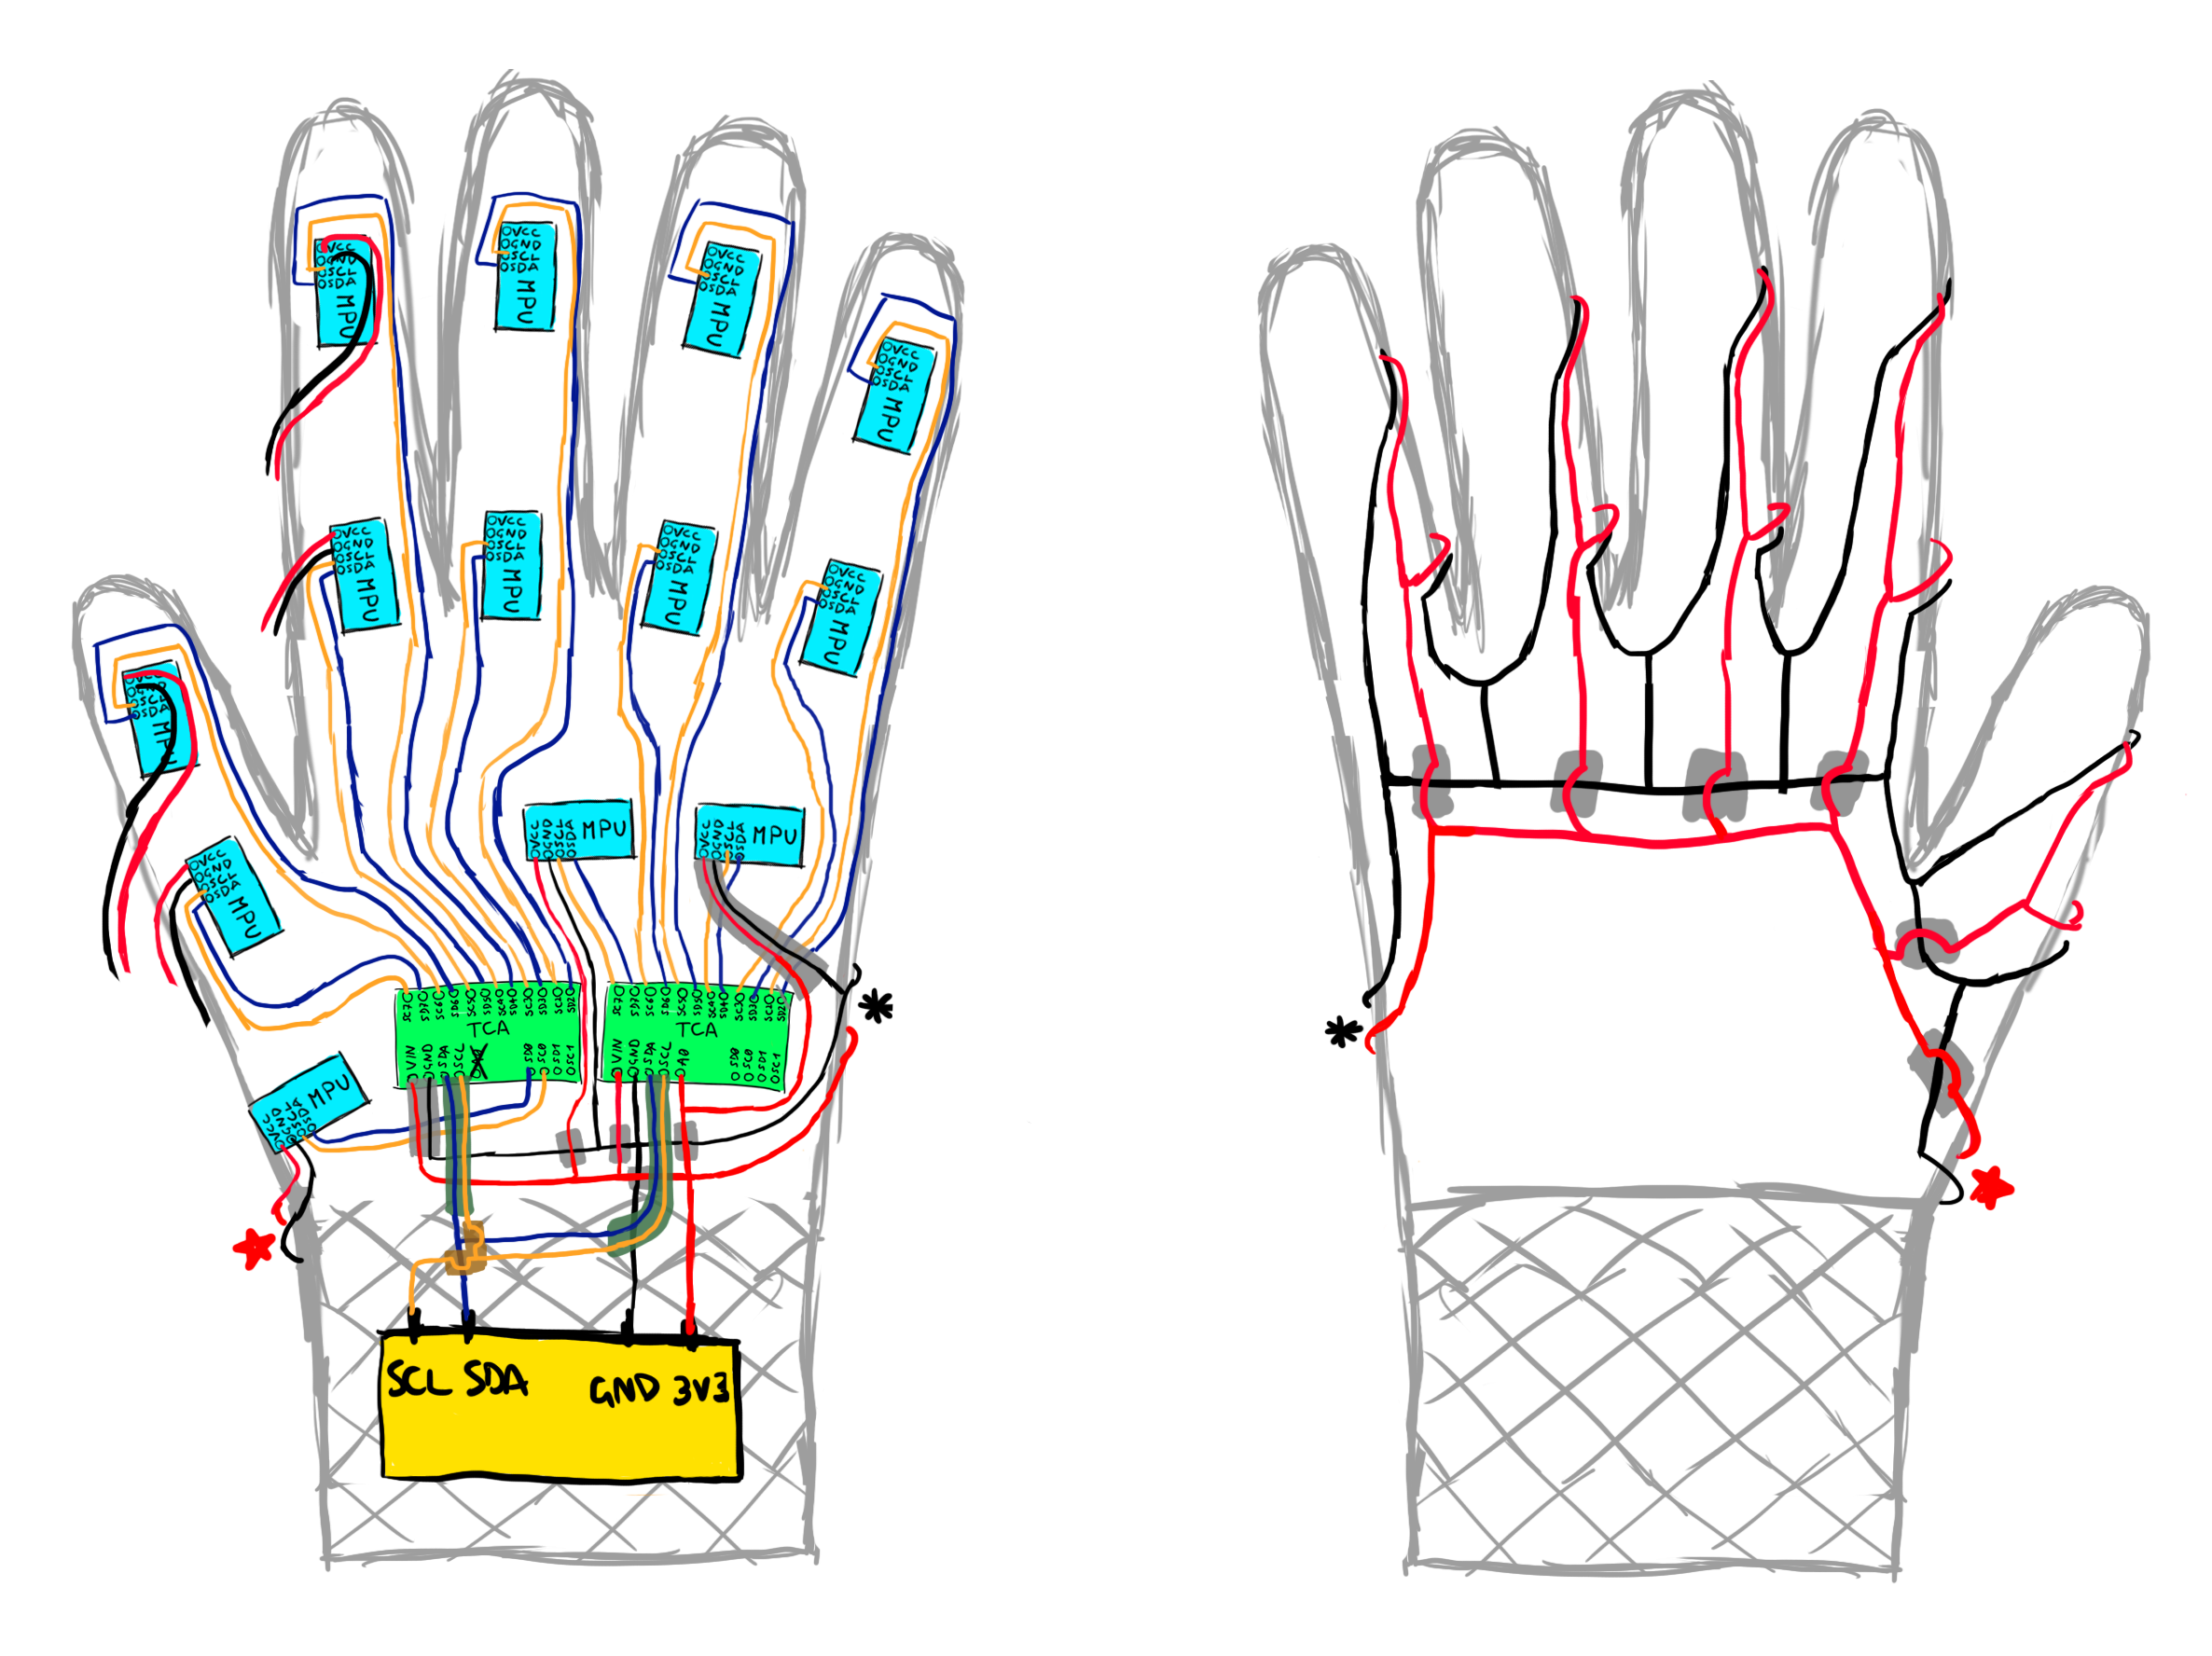
\includegraphics[scale=0.35]{immagini/guanto_schema.png}
    \centering
    \caption{V1 - schema dei collegamenti}
\end{figure}

\clearpage

\subsection{Secondo prototipo}

\begin{figure}[H]
    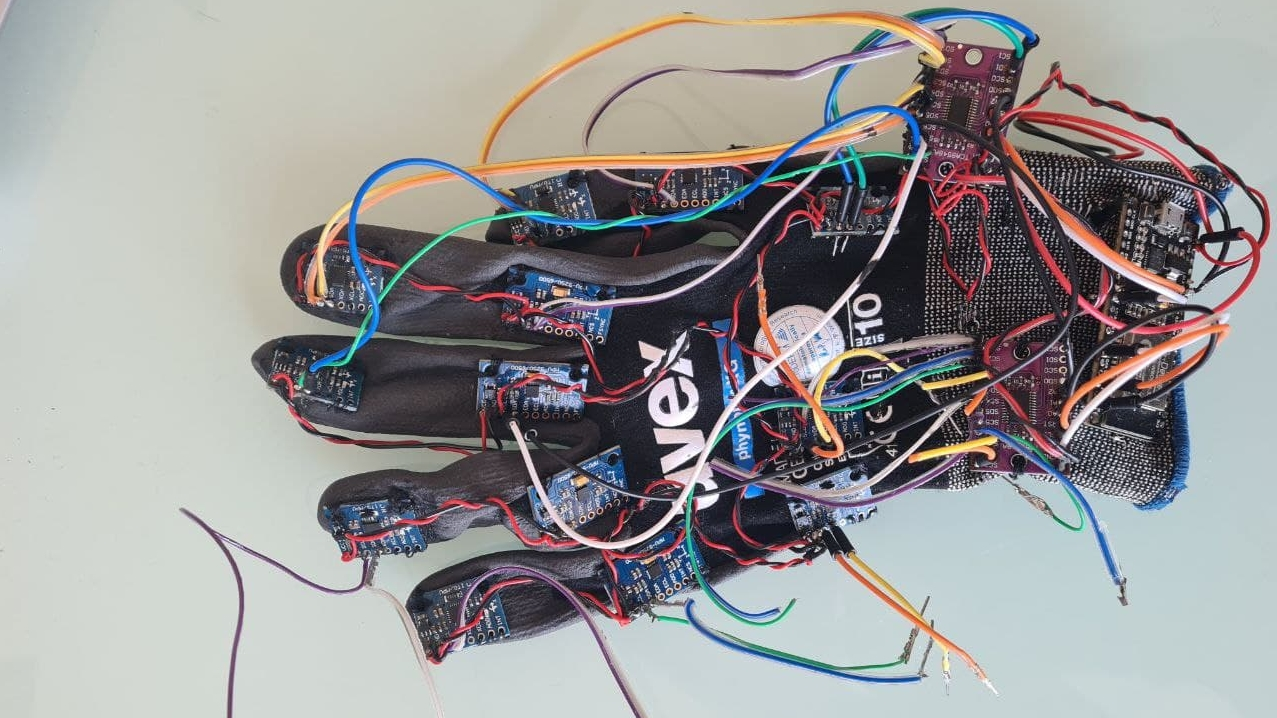
\includegraphics[scale=0.35]{immagini/prototipo2.jpg}
    \centering
    \caption{V2}
\end{figure}

Per il secondo prototipo del guanto si è abbandonata l'idea del filo per cucire conduttivo, sostituendolo con dei normali cavetti isolati, e in tal modo si è riusciti ad arrivare in una configurazione tale per cui tutte le IMU si accendessero senza problemi.\\

Ci sono stati tuttavia altri problemi imprevisti: alcuni collegamenti I2C perdevano sporadicamente segnale anche per minimi movimenti del guanto, e il programma di recezione dati riceveva zeri su tutte le misure dell'IMU; i cavi inoltre sono stati saldati e crimpati per avere collegamenti stabili ed evitare ulteriori errori, ma per effettuare operazioni di debugging è stato necessario tagliarli e ricollegarli più volte; infine, molte IMU usate avevano problemi di inizializzazione e su alcuni sensori restituivano il valore di fondoscala invece che la misura effettiva, facendo pensare dopo vari tentativi di debugging falliti che fosse l'IMU stessa ad essere non funzionante.\\

Per questi motivi si è passati a una terza versione del guanto, e poiché la probabilità di incorrere in problemi hardware aumenta proporzionalmente rispetto al numero di dispositivi utilizzati, si è quindi ritenuto necessario diminuire la complessità del progetto.

\clearpage

\subsection{Versione finale}

\begin{figure}[H]
    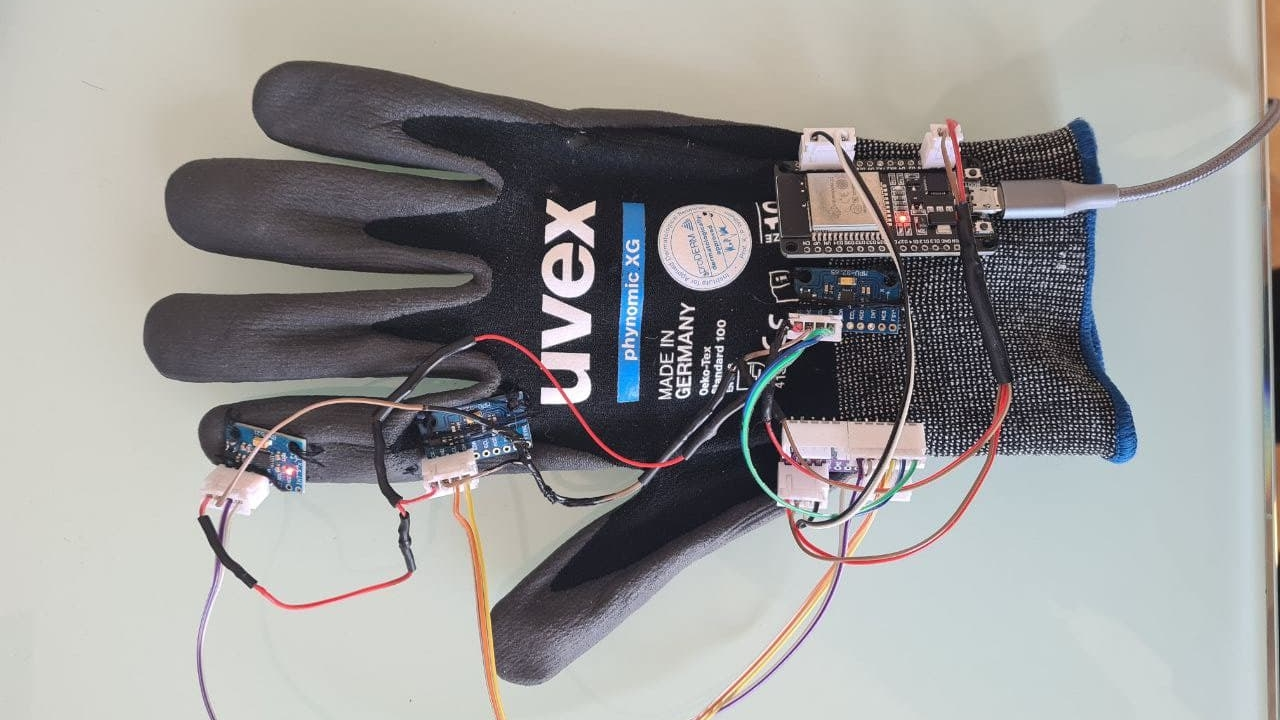
\includegraphics[scale=0.35]{immagini/prototipo3.jpg}
    \centering
    \caption{V3 - semplificato}
\end{figure}

La versione finale è quindi focalizzata su un solo dito, l'indice, e di conseguenza impiega molti meno dispositivi.\\

Tutti i dispositivi utilizzati sono stati testati in modo approfondito prima ancora di essere installati sul guanto, per assicurarsi che funzionasse correttamente.\\

Con questa versione non ci sono stati problemi, e ogni nuova IMU collegata è stata testata prima di connettere la successiva. I cavi invece di venire saldati direttamente sono stati collegati con degli header (JTS).
L'inserzione degli header JTS garantisce un collegamento solido, evitando problemi di connessioni instabili (molto presenti nel caso di I2C), ma allo stesso tempo consente di poterli scollegare e ricollegare in qualsiasi momento.\\

\clearpage
\section{Software di basso livello per invio dati}

La scheda ESP32 è stata programmata da Arduino: non sono state utilizzate librerie (a parte ovviamente \mcode{Wire.h}), ma ci si è rifatti a \cite{MPU6050_tockn} e \cite{MPU9250} come riferimento per la costruzione del programma.\\
Di seguito una breve panoramica del funzionamento.

\subsection{Setup}

Il programma inizia facendo un check di tutti i canali del multiplexer e inizializzando le IMU presenti.\\
Poiché i giroscopi potrebbero misurare angoli diversi da 0 all'avvio, è stata implementata la possibilità di calibrarli tramite la funzione \mcode{calc_gyro_offset()}, che richiede di lasciare l'IMU immobile per raccogliere misure di velocità angolari di cui poi verrà fatta la media, che sarà il bias che viene poi sottratto a ogni successiva lettura; questa funzione è attivabile e disattivabile tramite la variabile booleana \mcode{calibrate_gyro}.\\

Durante il setup viene mandato un segnale al magnetometro con la funzione \mcode{initAK8963()}, e se l'IMU in questione è una 9250 ad esso segue l'inizializzazione del magnetometro, mentre se è una 6050 si interrompe senza fare nulla.\\
Per le MPU-9250 è stata anche implementata la possibilità di calibrare i magnetometri tramite la funzione \mcode{calc_magn_hard_iron_soft_iron_offset()} per eliminare i bias soft-iron, dati da interferenze di materiali magnetici, e hard-iron, date da parti che generano un proprio campo magnetico presenti sulla scheda stessa (basti pensare al campo magnetico prodotto dalla corrente che scorre in un circuito); questa funzione è attivabile e disattivabile tramite la variabile booleana \mcode{calibrate_magn}.\\
Riferimenti sulla calibrazione del magnetometro in \cite{MPU9250}, \cite{ozyagcilar2012calibrating} e \cite{ozyagcilar2012implementing}.\\

\begin{figure}[H]
    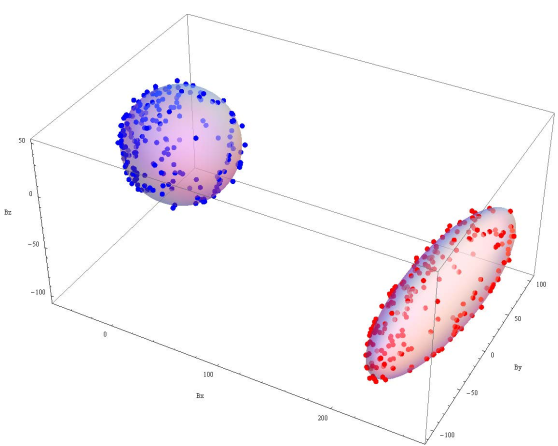
\includegraphics[scale=0.65]{immagini/distorsione campo magnetico confronto.PNG}
    \centering
    \caption{Campo magnetico corretto (sferico e centrato in $\overline{0}$) a sinistra, a confronto con campo magnetico distorto (bias hard-iron lo decentrano e bias sof-iron lo deformano) a destra.}
\end{figure}

Un'ultima funzione, normalmente disattivata, \mcode{I2C_scan()}, permette di effettuare uno scan di tutti i possibili address sul canale I2C per controllare quali dispositivi rispondono per ogni canale del multiplexer: tale funzione è stata particolarmente utile nelle fasi di sviluppo e debugging del progetto.\\

\subsection{Lettura dati}

Nel loop principale i dati vengono letti e stampati su seriale a ogni iterazione.\\

La funzione \mcode{read_data()} (che richiama la sotto-funzione \mcode{read_raw_data()}) consente di accedere ai registri di memoria delle IMU e ricostruire la giusta lettura, prima unendo i byte raw (high e low), e poi correggendo con apposite variabili date su datasheet o con le misure di bias trovate se sono state effettuate calibrazioni nella fase di setup.\\

La lettura dei dati delle IMU avviene a una frequenza di 400 kHz complessivi e quindi ogni IMU viene letta a circa 130 kHz. Ogni dato da leggere è composto da 8 bit e sono presenti 9 misure da leggere, conseguentemente 72 bit per ogni MPU.\\
La velocità del canale I2C risulta sufficiente per avere un buon aggiornamento della stima e un delay ridotto.\\


La funzione \mcode{print_data()} invece invia al seriale i dati letti, in modo che possano essere recepiti da PC ed elaborati nel filtro.


\clearpage
\section{Il filtro}

Per l'elaborazione dei dati ricevuti dalle IMU è stato utilizzato il filtro complementare, che unisce un'implementazione relativamente semplice a dei risultati di performance comparabili a filtri più complessi, come il filtro di Kalman.\\

Esso si basa su un processo di \textit{sensor fusion} con il raggiungimento di una stima degli angoli di roll, pitch e yaw tramite due diversi approcci, per poi unire i due contributi a meno di una costante complementare $\alpha$ che esprime il grado di fiducia nel corrispettivo sensore.\\

In particolare, nel progetto in questione si è fatto anche riferimento all'articolo \cite{KOTTATH2017574}, che applica un filtro complementare leggermente diverso da quello canonico.

\begin{figure}[H]
    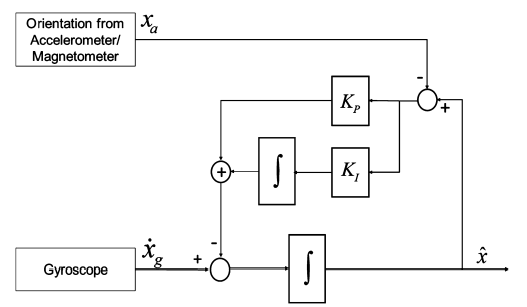
\includegraphics[scale=1]{immagini/filter.png}
    \centering
    \caption{Schema filtro complementare proposto}
\end{figure}

Nella prima parte, gli angoli vengono ottenuti dall'integrazione delle misure del giroscopio, paragrafo (\ref{Dati giroscopio}) equazioni (\ref{integr phi}) (\ref{integr theta}) e (\ref{integr psi}):\\

\begin{equation*}
    \begin{cases}
        \dot{\phi} = p + q \sin{\phi} \tan{\theta} + r \cos{\phi} \tan{\theta}\\
        \dot{\theta} = q \cos{\phi} - r \sin{\phi}\\
        \dot{\psi} = q \sin{\phi} \sec{\theta} + r \cos{\phi} \sec{\theta}
    \end{cases}
\end{equation*}\\

nella seconda parte, roll e pitch derivano da formule basate su considerazioni sulla gravità già discusse nel paragrafo (\ref{Dati accelerometro}) equazioni (\ref{eq phi roll acc}) e (\ref{eq theta pitch acc}); lo yaw, come già discusso nel paragrafo (\ref{Dati magnetometro}), necessita di un riferimento di \textit{heading} e quindi del magnetometro, paragrafo (\ref{Dati magnetometro}) equazione (\ref{eq psi yaw magn}):\\

\begin{equation*}
    \begin{cases}
        \phi_a = \tan^{-1} \begin{pmatrix} \frac{a_y}{a_z} \end{pmatrix}\\
        \theta_a = \tan^{-1} \begin{pmatrix} \frac{-a_x}{a_y \sin{\phi_a} \, + \, a_z \cos{\phi_a}} \end{pmatrix}\\
        \psi_m = \tan^{-1} \begin{pmatrix} \frac{m_x \sin{\phi_a} \, - \, m_y \cos{\phi_a}}{m_x \cos{\theta_a} \, + \, m_y \sin{\theta_a} \sin{\phi_a} \, + \, m_z \sin{\theta_a} \cos{\phi_a}} \end{pmatrix}
    \end{cases}
\end{equation*}\\


Infine quindi tali stime basate sui singoli sensori vengono unite: la formula classica (\cite{ahrs}, quaternioni) è
\begin{equation}
    \hat{q} = \alpha \, q_g + (1 - \alpha) \, q_{am}
\end{equation}

che in seguito è stata ripresa ed espansa (\cite{KOTTATH2017574}) come
\begin{equation}
    \hat{x}_{new} = \frac{1}{s} \begin{bmatrix} \dot{x}_g + (K_p + \frac{K_I}{s}) (x_{am} - \hat{x}) \end{bmatrix}
\end{equation}

e che rivista e semplificata ($K_I = 0$) diventa
\begin{equation}
    \hat{x}_{new} = \frac{1}{s} \begin{bmatrix} \alpha \, \dot{x}_g + (1 - \alpha) (x_{am} - \hat{x}) \end{bmatrix}
\end{equation}

dove 
\begin{equation}
    \dot{x}_g = \columnvector{\dot{\phi} \\ \dot{\theta} \\ \dot{\psi}} \quad , \quad x_{am} = \columnvector{\phi_a \\ \theta_a \\ \psi_m}
\end{equation}\\

$\hat{x}_{new}$ è la stima finale degli angoli di roll pitch e yaw, $\hat{x}$ è la stima allo step precedente, $\dot{x}_g$ sono le velocità angolari ricavate dai giroscopi dopo le correzioni di rotazione, e $x_{am}$ sono le misure ricavate da accelerometro e magnetometro.\\

La formula finale quindi risente di entrambi i metodi, dove la variabile proporzionale $K_p$ è stata riconvertita in $\alpha$.\\
È stato poi notato sperimentalmente che il valore migliore per $\alpha$ fosse più vicino a 1, e si assestasse su 0.9.\\

Le funzioni di filtraggio sono presenti nel codice python, in particolare il lavoro viene svolto dalla funzione \mcode{Complementary2eul()}.

\begin{figure}[H]
    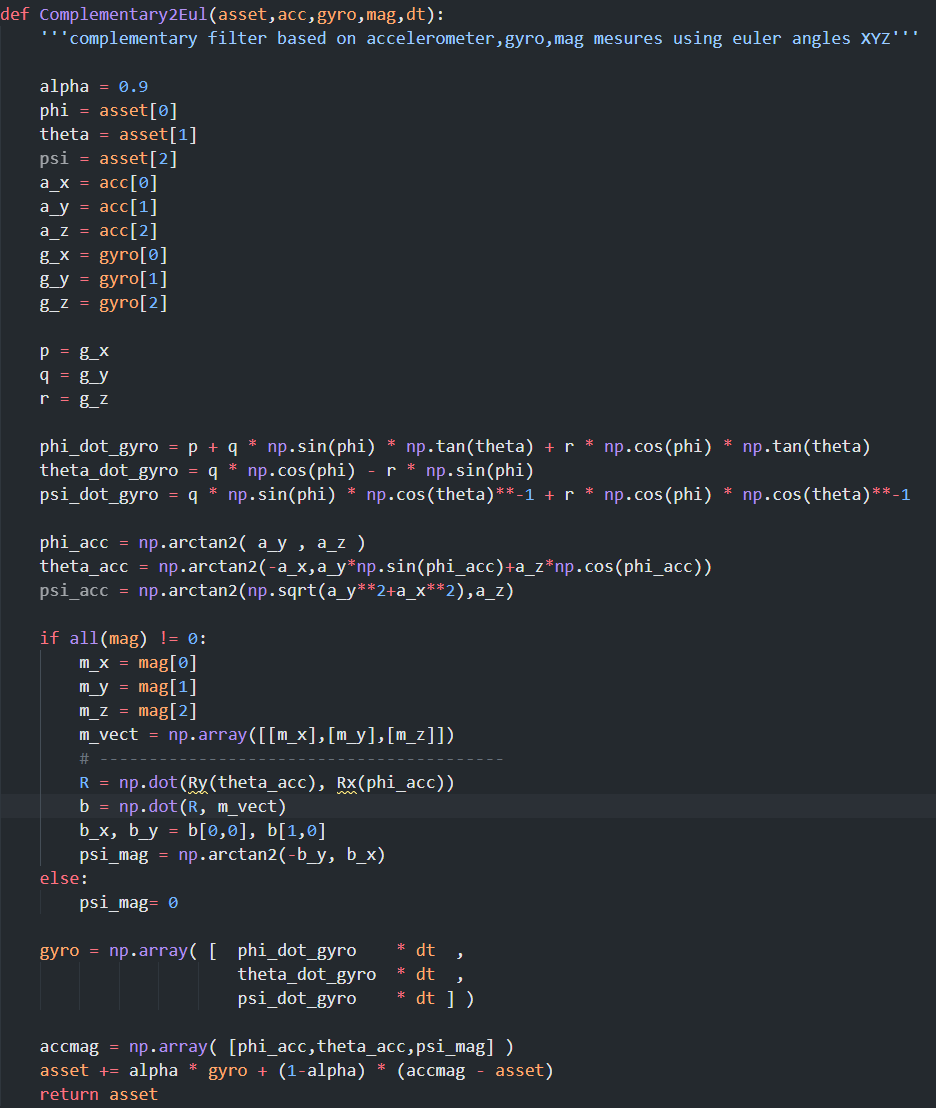
\includegraphics[scale=0.6]{immagini/filtercode.png}
    \centering
    \caption{Codice del filtro complementare.}
\end{figure}

\clearpage
\section{Rappresentazione virtuale}

\subsection{Pybullet/URDF}

Inizialmente si era pensato di utilizzare la libreria Python Pybullet per creare l'ambiente tridimensionale, e un file .urdf.xacro per generare la mano.\\

Qui vengono riportate alcune immagini di tale prototipo virtuale.\\

\begin{figure}[htb] %width=0.6\linewidth
    \centering
    \subfloat
        {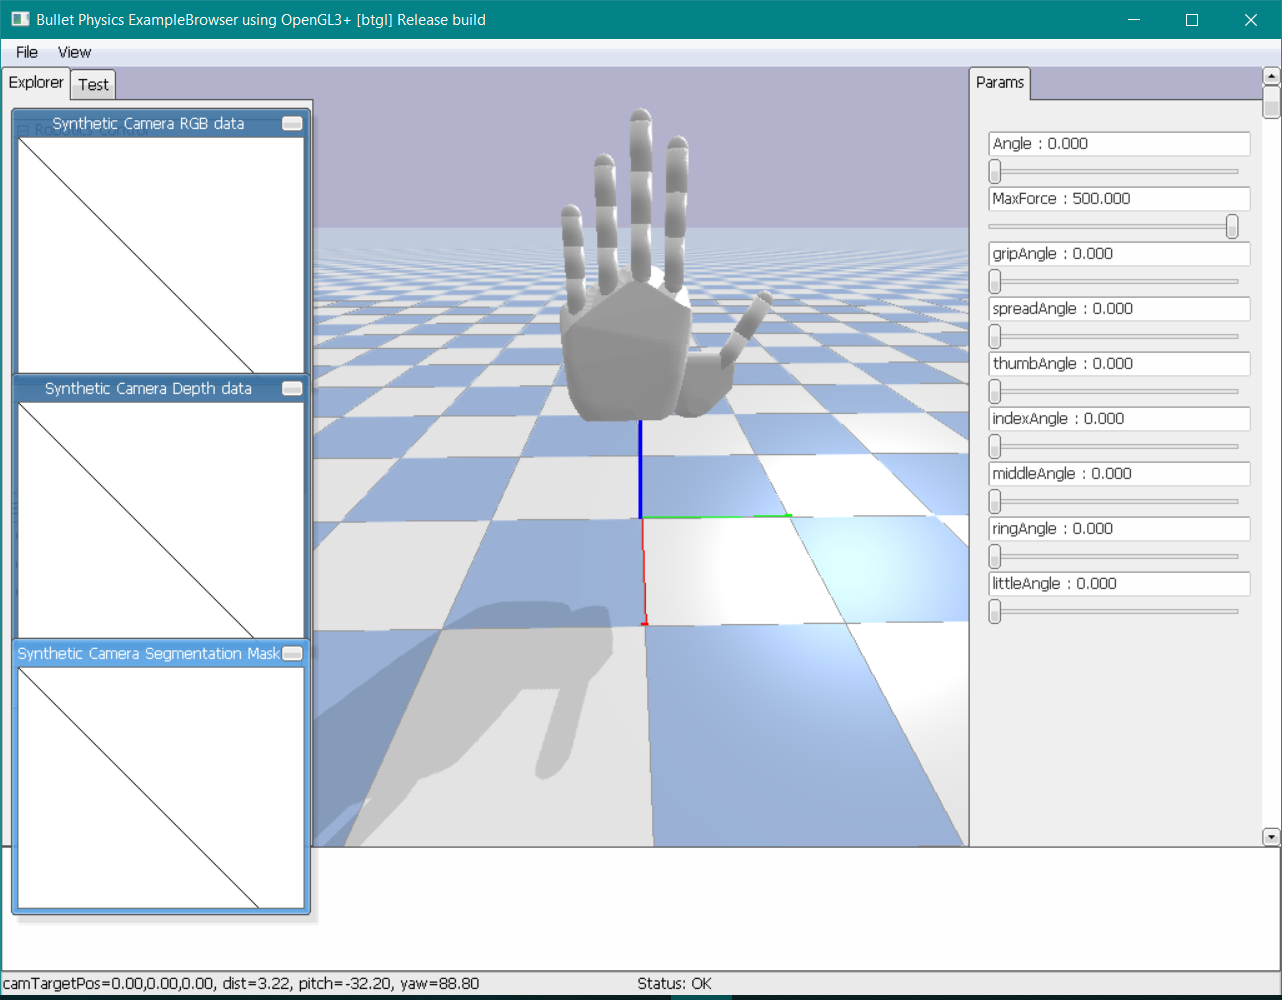
\includegraphics[height=.27\textheight]{immagini/pybullet urdf.PNG}}\
    \subfloat
        {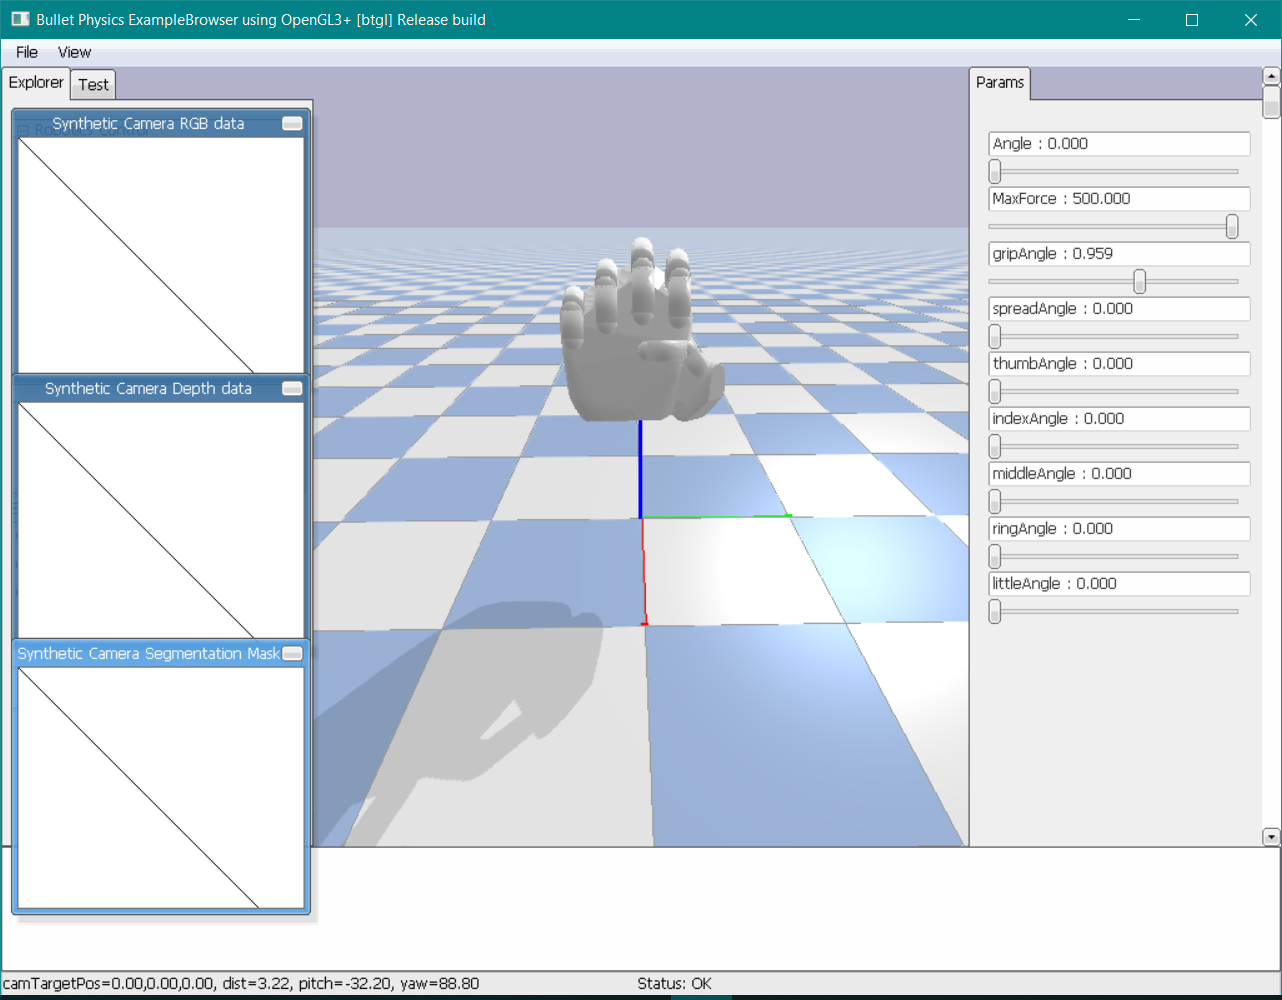
\includegraphics[height=.27\textheight]{immagini/pybullet urdf grip.PNG}}
    %\caption{}
\end{figure}

\begin{figure}[htb] %width=0.6\linewidth
    \centering
    \subfloat
        {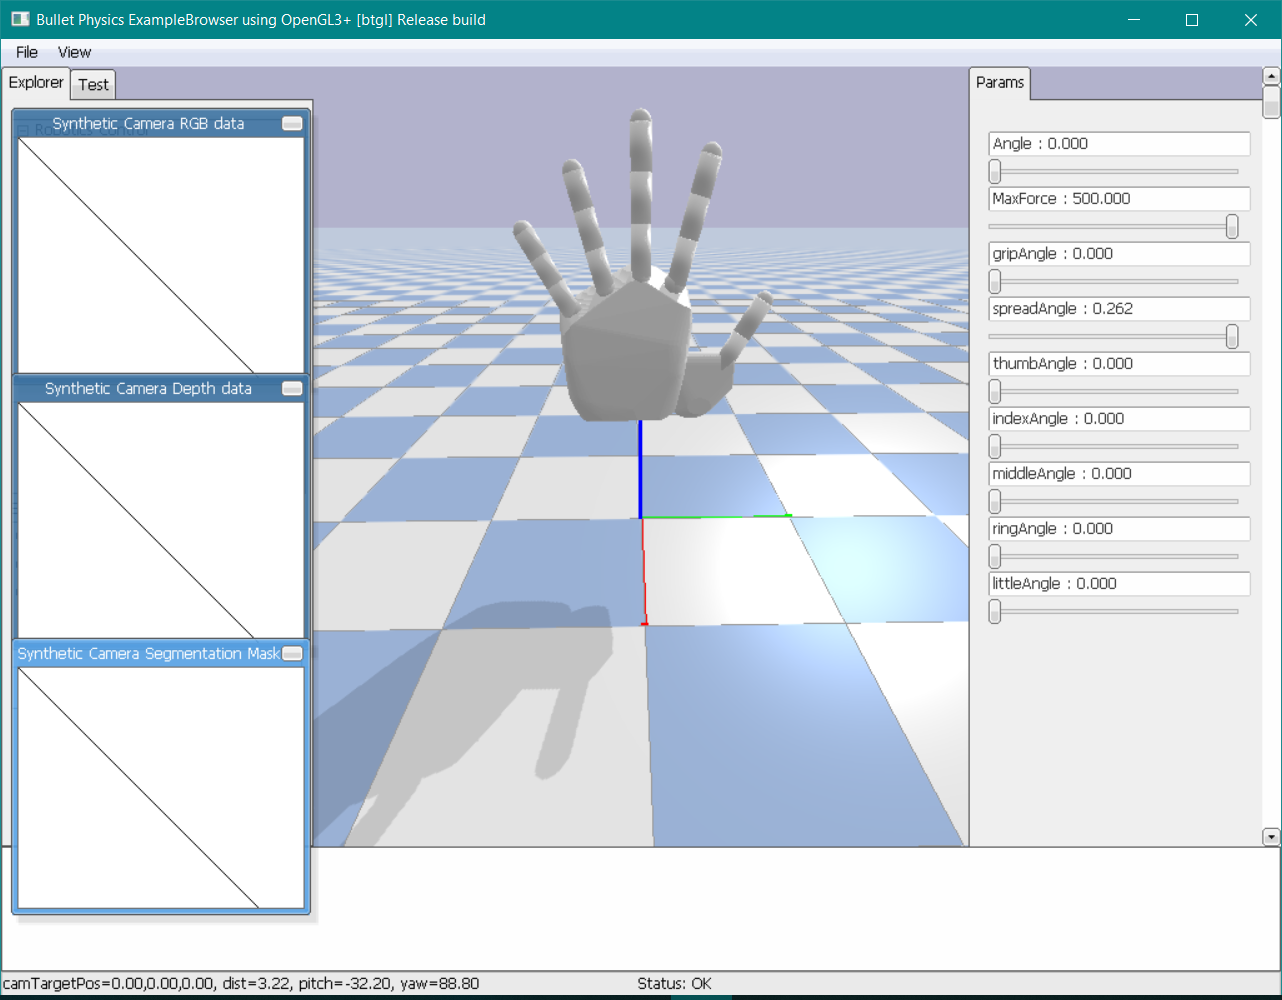
\includegraphics[height=.27\textheight]{immagini/pybullet urdf spread.PNG}}\
    \subfloat
        {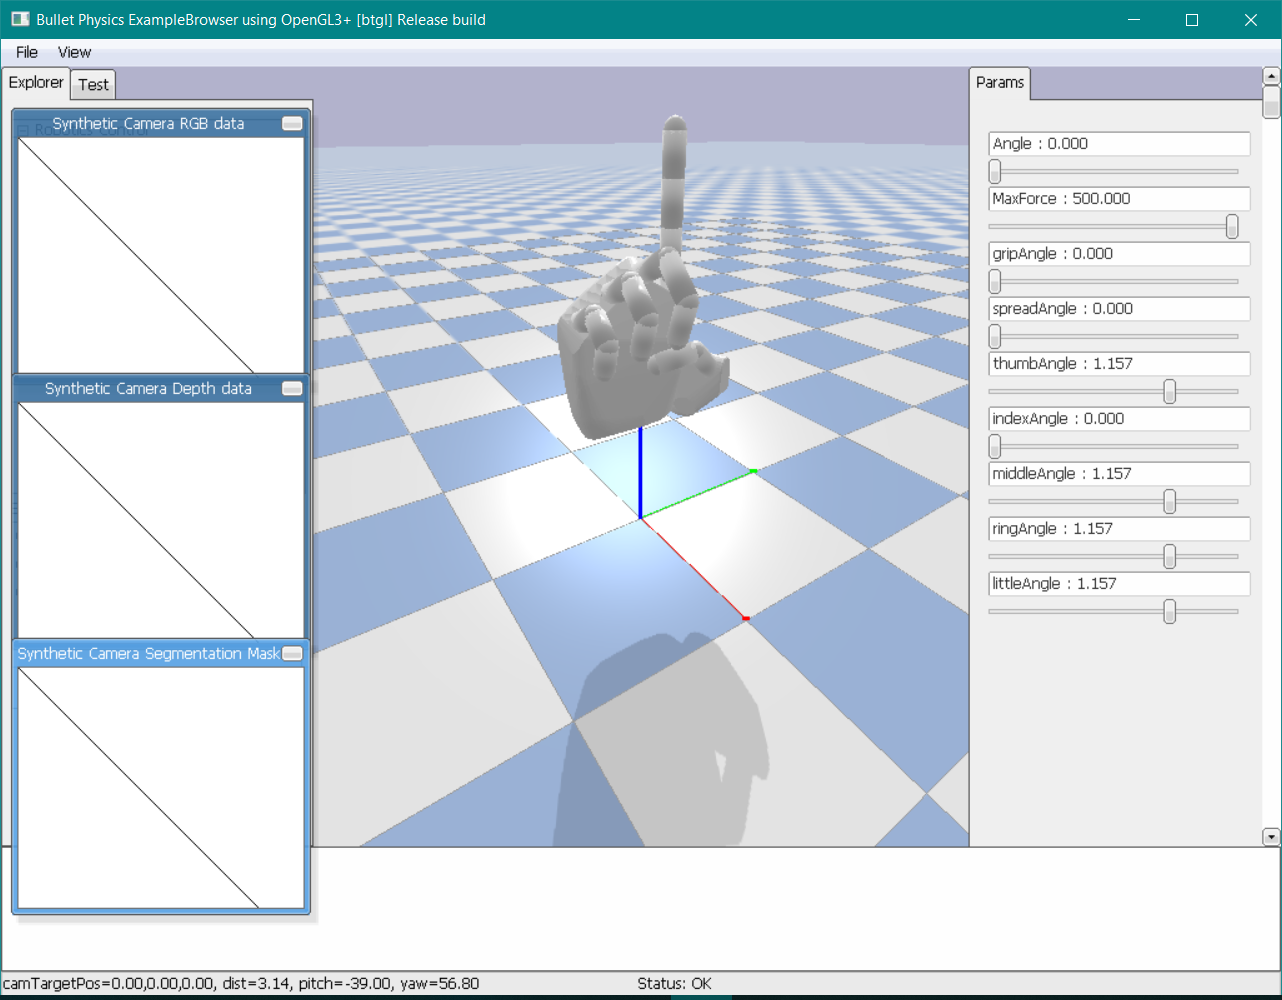
\includegraphics[height=.27\textheight]{immagini/pybullet urdf point.PNG}}
    %\caption{}
\end{figure}

\clearpage

\subsection{Unity}

In seguito si è passati all'utilizzo di Unity e alla mano virtuale dell'Oculus Rift.\\

\begin{figure}[H]
    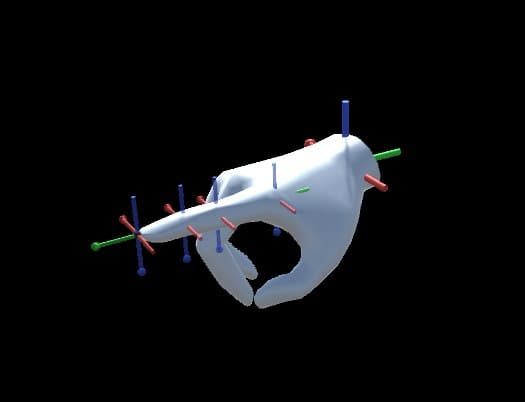
\includegraphics[scale=1]{immagini/vrhandunity.jpg}
    \centering
    \caption{Visualizzazione della mano su Unity}
\end{figure}

\\\\

\subsubsection{Elaborazione dei dati}

Una volta filtrati i dati tramite la batteria di stimatori d'assetto, vengono inviate le stime a una batteria di stimatori di orientazione relativa. Essi hanno lo scopo di calcolare l'angolo di giunto delle falangi della mano prendendo in ingresso l'assetto di 2 link successivi e calcolandone la rotazione relativa.

\begin{figure}[H]
    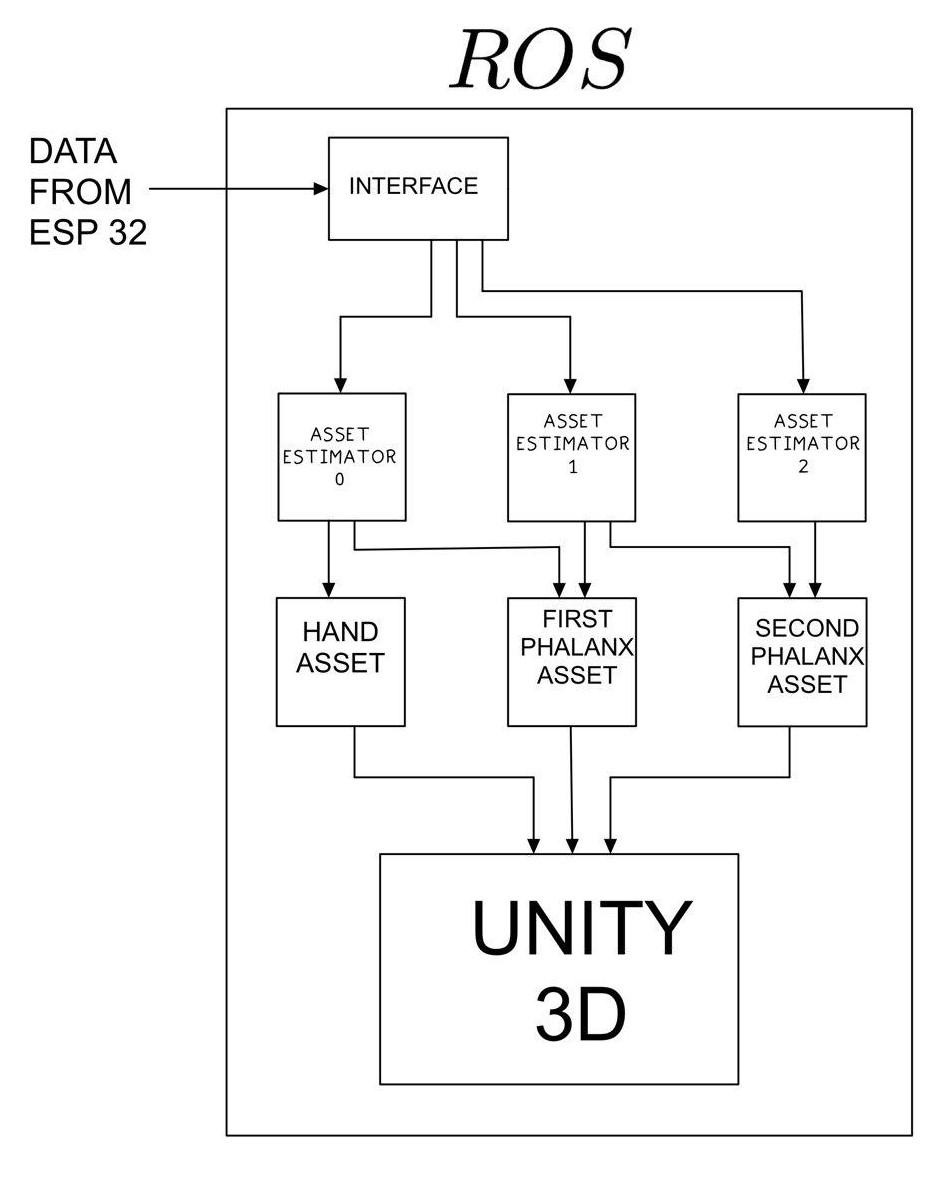
\includegraphics[scale=0.2]{immagini/unity.jpg}
    \centering
    \caption{Schema di stima e di calcolo di rotazioni relative}
\end{figure}

\begin{equation}
    T_{01_{rel}} = T_0(\theta_0,\phi_0,\psi_0)^{-1} \cdot T_1(\theta_1,\phi_1,\psi_1)
    \label{slerp}
\end{equation}

\begin{equation}
    T_{12_{rel}} = T_1(\theta_1,\phi_1,\psi_1)^{-1} \cdot T_2(\theta_2,\phi_2,\psi_2)
    \label{slerp}
\end{equation}\\

Dalla matrice di rotazione relativa possiamo estrapolare gli angoli di Eulero:
\begin{equation}
    R = T_{rel} =  \left(\begin{array}{ccc}
    r_{11}  & r_{12}  & r_{13} \\
    r_{21}  & r_{22}  & r_{23} \\
    r_{31}  & r_{32}  & r_{33} 
    \end{array}\right)
    \label{slerp}
\end{equation}\\\\
\begin{equation}
    phi = atan2(r_{23},r_{33})
\end{equation}\\\\
\begin{equation}
    theta = - arcsin(r_{13})
\end{equation}\\\\
\begin{equation}
    psi = atan2(r{12},r_{11})
\end{equation}\\

Una volta calcolati gli angoli di giunto vengono inviati tramite ROS2 i messaggi relativi ai singoli angoli di giunto e all'assetto della mano completa a un software di visualizzazione grafica. \\
Per validare i risultati è stata impostata una simulazione su Unity3D che ci permette di visualizzare in real time i risultati della stima d'asetto tramite codice C\# integrato in Unity. \\\\
Una volta che le stime degli angoli di giunto erano a disposizione su unity, i valori sono stati trasformati in quaternioni (i software di grafica 3D ne fanno uso estensivo visto il minor costo computazionale) e tra un campione e il successivo viene eseguita una interpolazione SLERP (spherical linear interpolation) di velocità programambile.\\
Essa è particolarmente indicata per interpolare grandezze di tipo angolare e migliora il risultato rendendo l'animazione più fluida e meno rumorosa.\\

\begin{equation}
    q = \begin{bmatrix}[1.5] \cos(\frac{\phi}{2})\cos(\frac{\theta}{2})\cos(\frac{\psi}{2}) + \sin(\frac{\phi}{2})\sin(\frac{\theta}{2})\sin(\frac{\psi}{2})\\ \sin(\frac{\phi}{2})\cos(\frac{\theta}{2})\cos(\frac{\psi}{2}) - \cos(\frac{\phi}{2})\sin(\frac{\theta}{2})\sin(\frac{\psi}{2})\\ \cos(\frac{\phi}{2})\sin(\frac{\theta}{2})\cos(\frac{\psi}{2}) + \sin(\frac{\phi}{2})\cos(\frac{\theta}{2})\sin(\frac{\psi}{2})\\ \cos(\frac{\phi}{2})\cos(\frac{\theta}{2})\sin(\frac{\psi}{2}) - \sin(\frac{\phi}{2})\sin(\frac{\theta}{2})\cos(\frac{\psi}{2}) \end{bmatrix}
\end{equation}

\begin{equation}
    Slerp(q_1,q_2,u) = q_1\cdot(q_1^{-1} \cdot q_2)^{u}
    \label{slerp}
\end{equation}

\begin{figure}[H]
    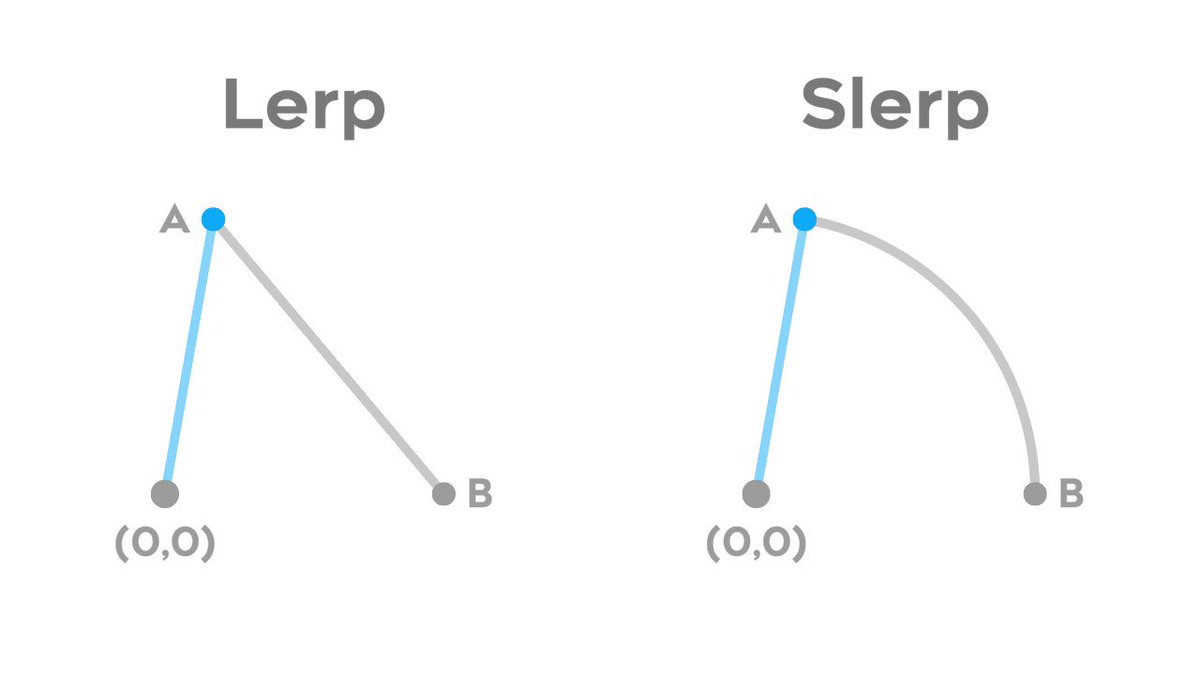
\includegraphics[scale=0.3]{immagini/lerp.jpg}
    \centering
    \caption{lerp - slerp piano}
\end{figure}

\begin{figure}[H]
    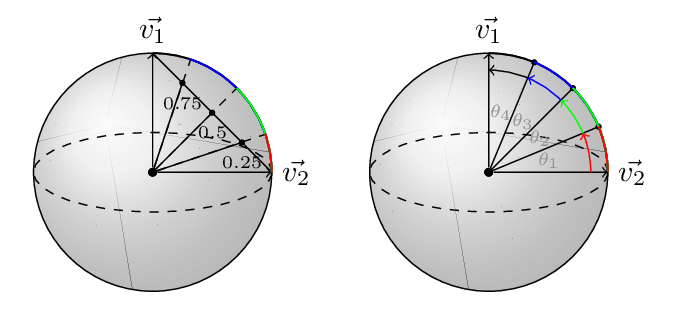
\includegraphics[scale=0.7]{immagini/slerplerp.png}
    \centering
    \caption{lerp - slerp differenza sulla sfera del quaternione unitario}
\end{figure}

È stata importata una mesh 3D di una mano da Oculus Rift, e ad essa sono stati agganciati sistemi di riferimento coerenti con quelli delle IMU.
I sistemi di riferimento vengono visualizzati secondo lo schema RGB - XYZ e sono solidali con i giunti presenti nella mano virtuale.

\begin{figure}[H]
    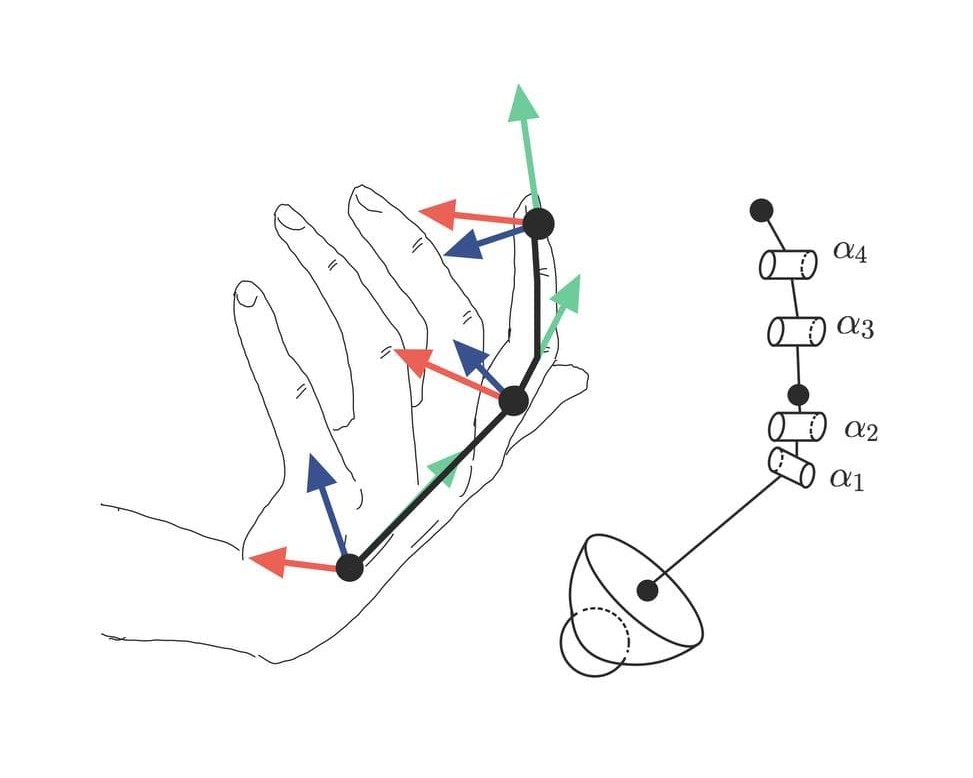
\includegraphics[scale=0.45]{immagini/kinematics_chain.jpg}
    \centering
    \caption{Catena cinematica.}
\end{figure}

Per la validazione dei risultati di stima abbiamo fatto uso esclusivamente di considerazioni di \textit{motion tracking}: muovendo il guanto, abbiamo considerato buona la stima quando la mano virtuale ne seguiva il movimento.

Per via delle convenzioni utilizzate al filtro e quelle usate da Unity la validità della simulazione risiede tra angoli compresi tra 0 e 180 gradi. Sforando questi angoli si hanno dei cambi di orientazione della mano.
Data la stima eccessivamente imprecisa dell'angolo $\alpha_1$ esso è stato mantenuto a 0.\\

\clearpage

\begin{figure}
 \centering
 \begin{subfigure}[ht]{0.3\textwidth}
     \centering
     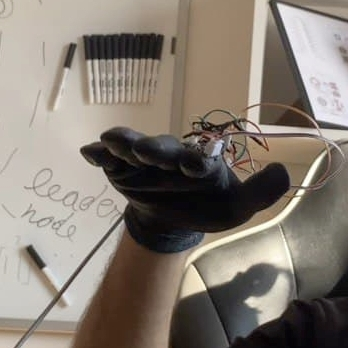
\includegraphics[width=5cm,height=5cm]{immagini/confronto/1.jpg}
     \caption{}
 \end{subfigure}
 \begin{subfigure}[ht]{0.3\textwidth}
     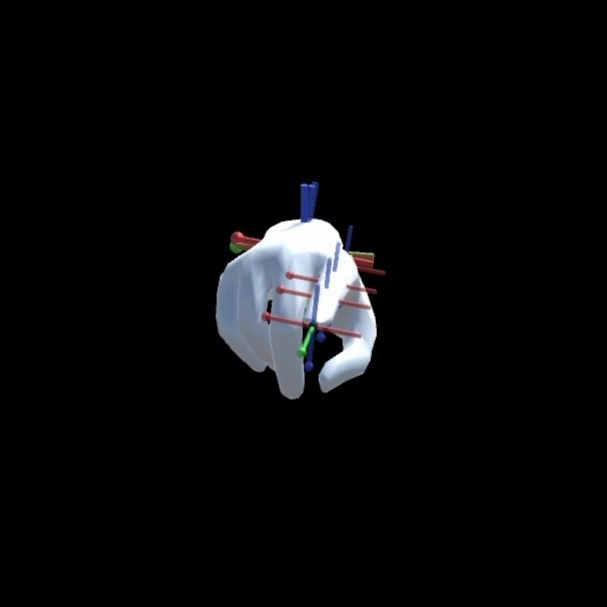
\includegraphics[width=5cm,height=5cm]{immagini/confronto/1_sym.jpg}
     \caption{}
 \end{subfigure}
 \caption{}
\end{figure}

\begin{figure}
 \centering
 \begin{subfigure}[ht]{0.3\textwidth}
     \centering
     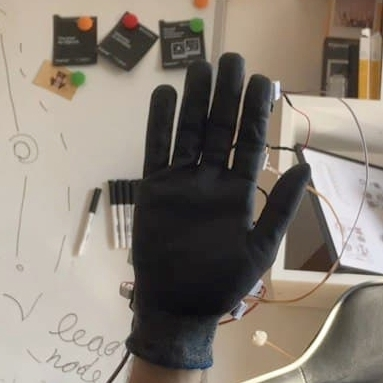
\includegraphics[width=5cm,height=5cm]{immagini/confronto/2_real.jpg}
     \caption{}
 \end{subfigure}
 \begin{subfigure}[ht]{0.3\textwidth}
     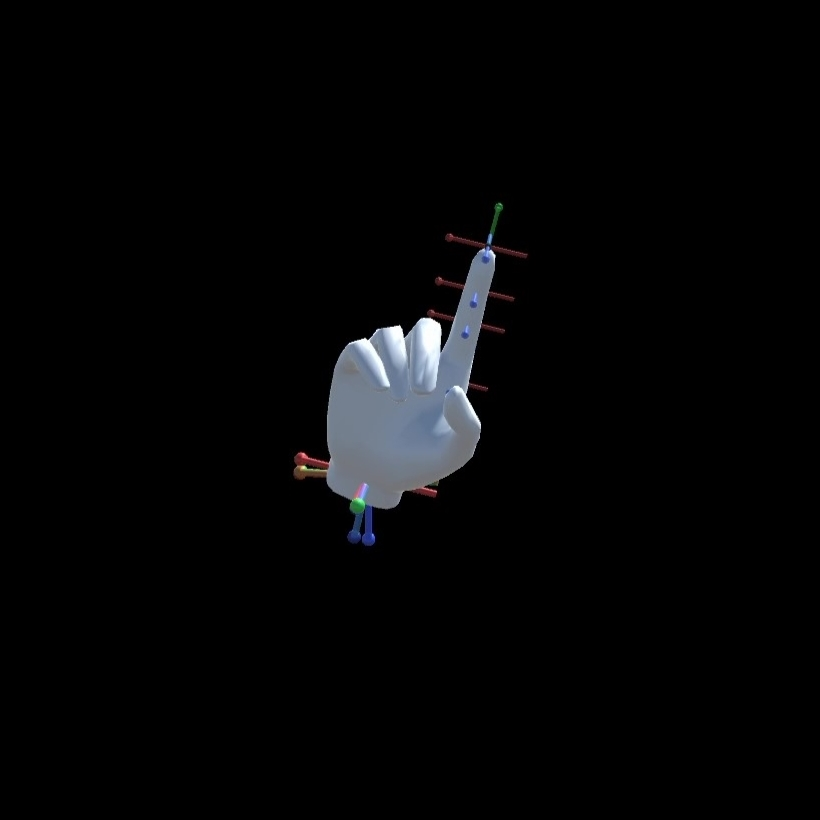
\includegraphics[width=5cm,height=5cm]{immagini/confronto/2_sym.jpg}
     \caption{}
 \end{subfigure}
 \caption{}
\end{figure}

\begin{figure}
 \centering
 \begin{subfigure}[ht]{0.3\textwidth}
     \centering
     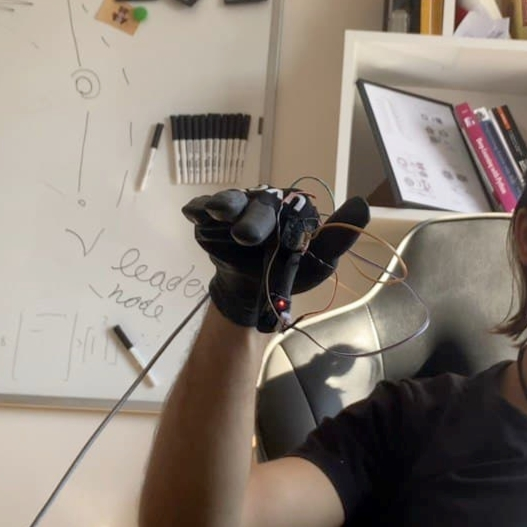
\includegraphics[width=5cm,height=5cm]{immagini/confronto/3_real.jpg}
     \caption{}
 \end{subfigure}
 \begin{subfigure}[ht]{0.3\textwidth}
     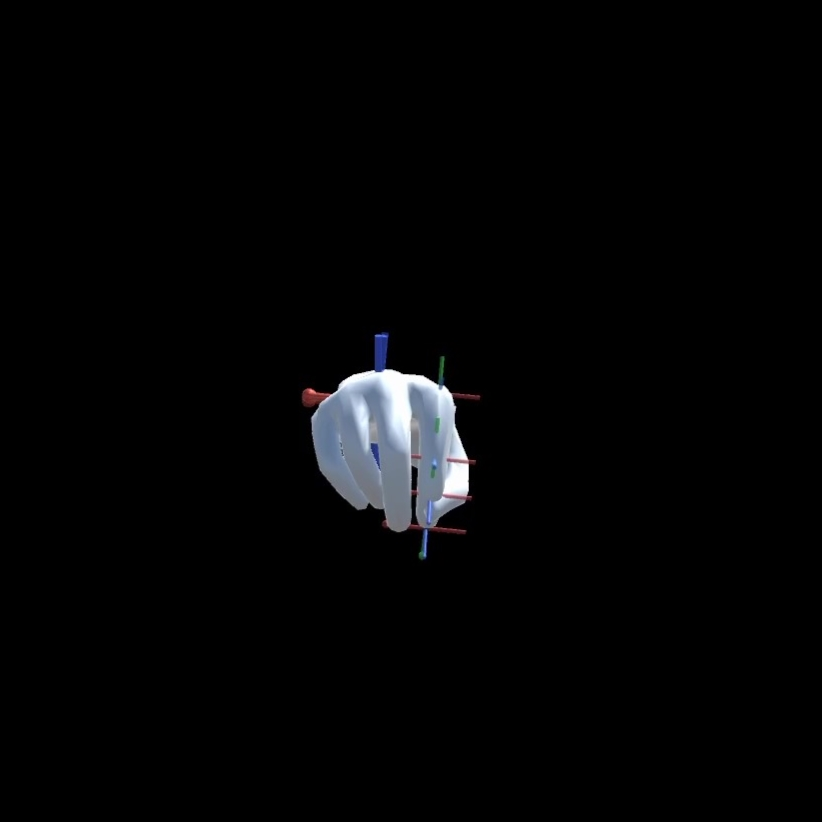
\includegraphics[width=5cm,height=5cm]{immagini/confronto/3_sym.jpg}
     \caption{}
 \end{subfigure}
 \caption{}
\end{figure}

\begin{figure}
 \centering
 \begin{subfigure}[ht]{0.3\textwidth}
     \centering
     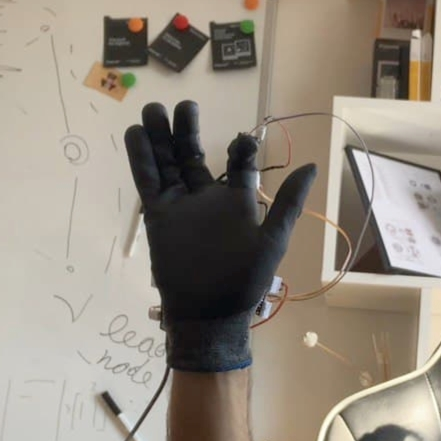
\includegraphics[width=5cm,height=5cm]{immagini/confronto/4_real.jpg}
     \caption{}
 \end{subfigure}
 \begin{subfigure}[ht]{0.3\textwidth}
     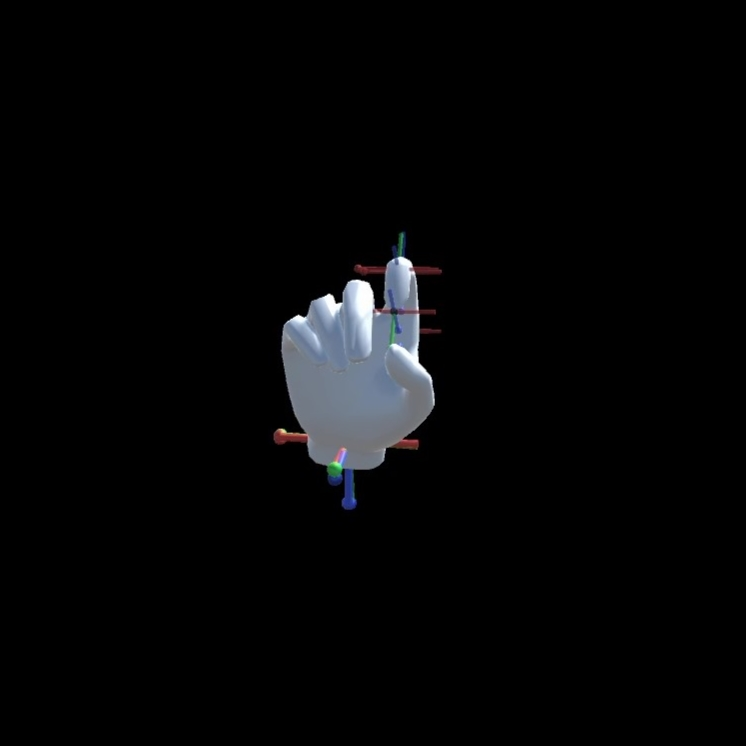
\includegraphics[width=5cm,height=5cm]{immagini/confronto/4_sym.jpg}
     \caption{}
 \end{subfigure}
 \caption{}
\end{figure}

\begin{figure}
 \centering
 \begin{subfigure}[ht]{0.3\textwidth}
     \centering
     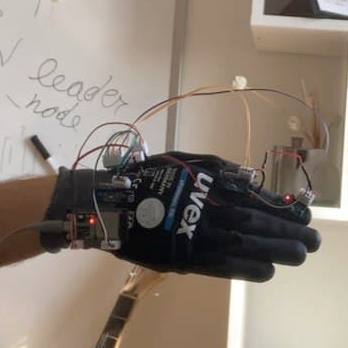
\includegraphics[width=5cm,height=5cm]{immagini/confronto/5_real.jpg}
     \caption{}
 \end{subfigure}
 \begin{subfigure}[ht]{0.3\textwidth}
     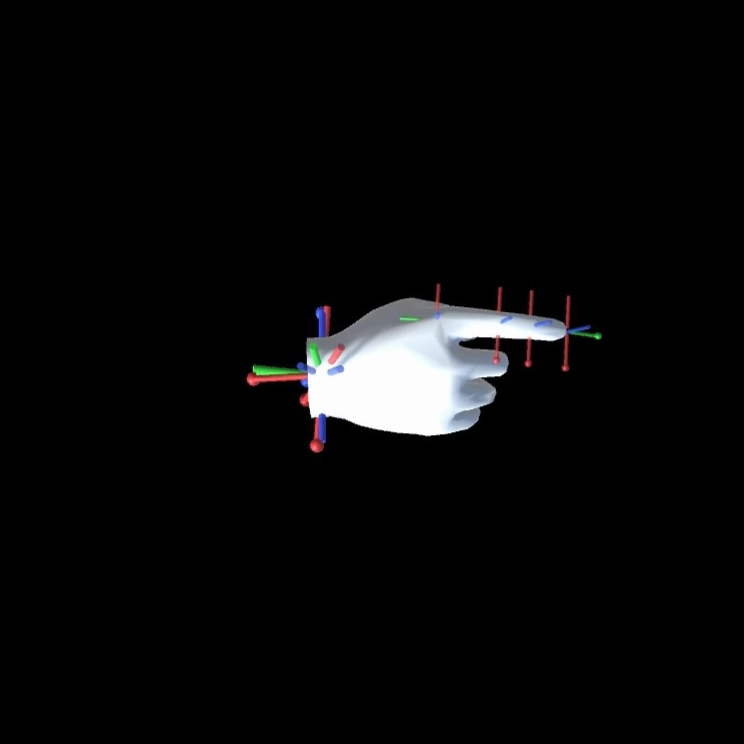
\includegraphics[width=5cm,height=5cm]{immagini/confronto/5_sym.jpg}
     \caption{}
 \end{subfigure}
 \caption{}
\end{figure}

\begin{figure}
 \centering
 \begin{subfigure}[ht]{0.3\textwidth}
     \centering
     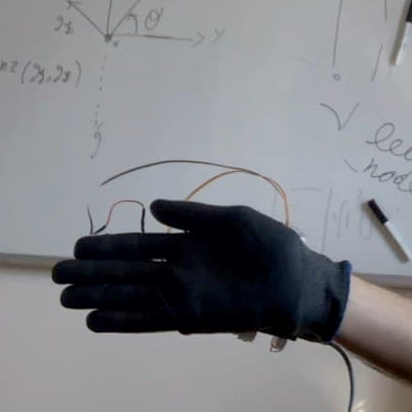
\includegraphics[width=5cm,height=5cm]{immagini/confronto/6_real.jpg}
     \caption{}
 \end{subfigure}
 \begin{subfigure}[ht]{0.3\textwidth}
     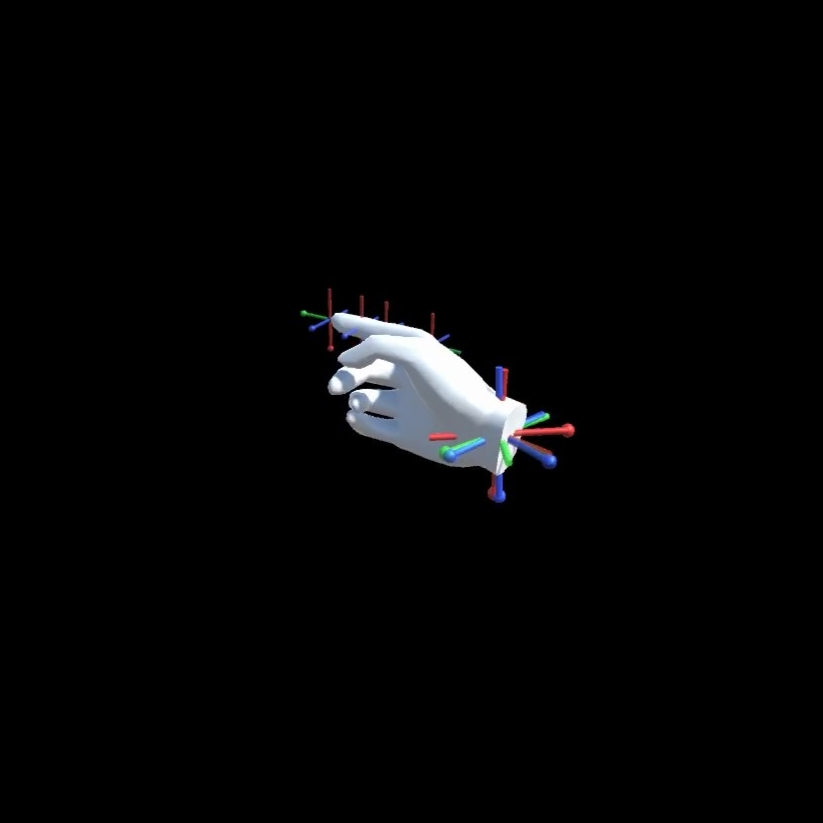
\includegraphics[width=5cm,height=5cm]{immagini/confronto/6_sym.jpg}
     \caption{}
 \end{subfigure}
 \caption{}
\end{figure}

\begin{figure}
 \centering
 \begin{subfigure}[ht]{0.3\textwidth}
     \centering
     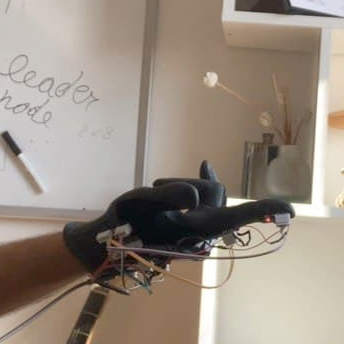
\includegraphics[width=5cm,height=5cm]{immagini/confronto/7_real.jpg}
     \caption{}
 \end{subfigure}
 \begin{subfigure}[ht]{0.3\textwidth}
     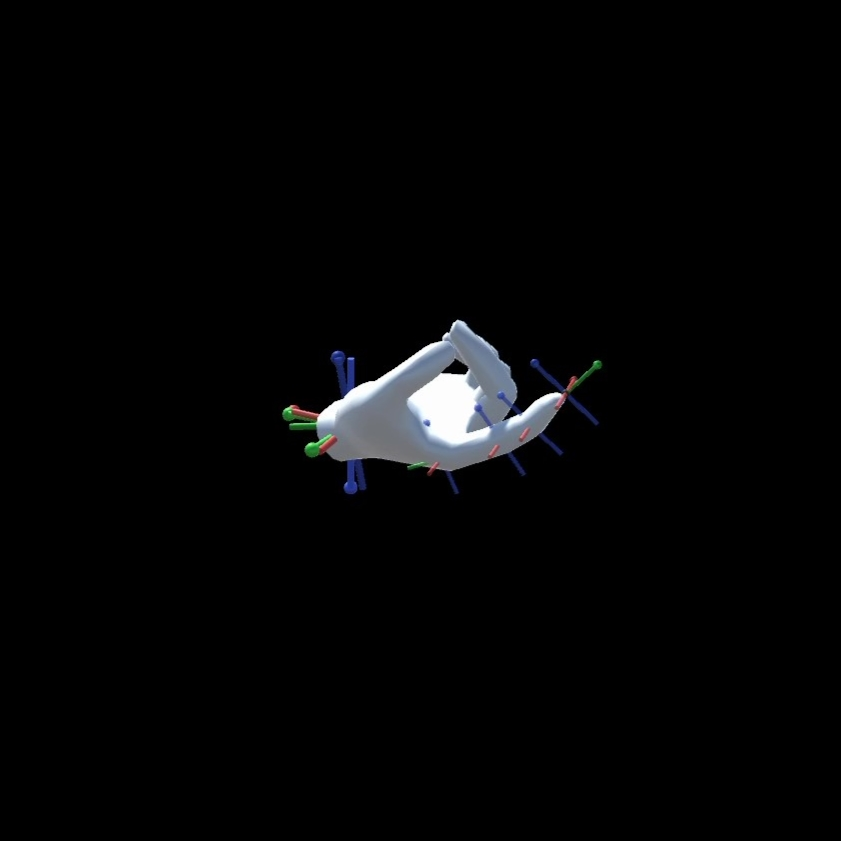
\includegraphics[width=5cm,height=5cm]{immagini/confronto/7_sym.jpg}
     \caption{}
 \end{subfigure}
 \caption{}
\end{figure}

\begin{figure}
 \centering
 \begin{subfigure}[ht]{0.3\textwidth}
     \centering
     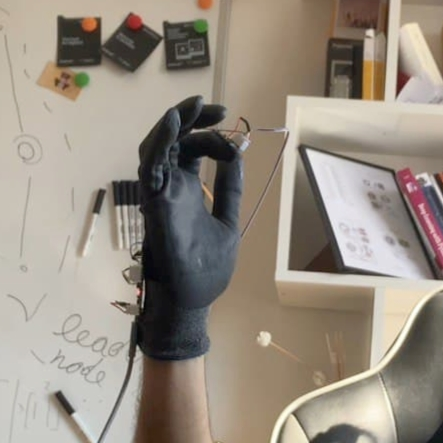
\includegraphics[width=5cm,height=5cm]{immagini/confronto/8_real.jpg}
     \caption{}
 \end{subfigure}
 \begin{subfigure}[ht]{0.3\textwidth}
     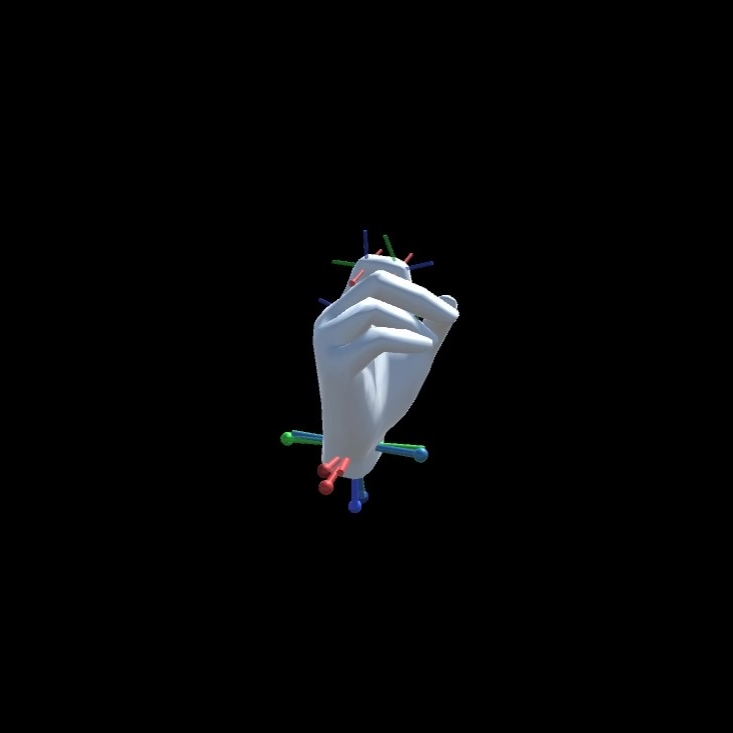
\includegraphics[width=5cm,height=5cm]{immagini/confronto/8_sym.jpg}
     \caption{}
 \end{subfigure}
 \caption{}
\end{figure}


\clearpage
\section{Conclusioni}

Nella simulazione le dita sono state piegate a pugno cosi da poter visualizzare adeguatamente la posizione del dito.\\

Sono stati fatti dei test filmando la mano e la relativa animazione e catturandone dei frame in contemporanea cosi da poterle mettere a confronto.\\

Come possiamo vedere dalle figure la posizione della mano virtuale rispecchia quella della mano reale e anche la posizione del dito virtuale rispecchia adeguatamente quella del dito reale per ogni posizione della mano.\\\\


\clearpage

\printbibliography

\end{document}



